\chapter{Nonequilibrium Monte-Carlo Methods}

\section{The Description of Irreversible Processes}
The statistical mechanics of irreversible processes is concerned with the
understanding of the following two observed facts \cite{vanKampenFund}:
Consider a collection of similar particles, e.g. atoms or molecules.

(i) On a microscopic level the equations of motion of all individual particles
are determined are determined completely by the familiar equations of motions
of classical mechanics (Newton's equations) or o quantum mechanics
(Schr\"odinger's equation). These equations are symmetric with respect to past
and future.

(ii) In avery rough and incomplete way the collection of particles may be
described by a small numer of macroscopic variables. These variables obey in a
selfconsistent way 
deterministic phenomenological differential equations (the balance equations) 
which are distinguish between past and future.

The problems is that there seems not to be a rigorous derivation of the
macroscopic irreversible equations form the reversible microscopic ones.
The task of statistical mechanics of irreversible processes  is to build an
approximate bridge beteween the microscopic description and the macroscopic
one. In particular, the most interesting question is: Where does the
irreversibility get in the description?

It seems to be appropriate to introduce an intermediate level of description
bewteen the microscopic and the macroscopic equations. The formal setting for
this description is the master equation, which as we already know has the
general form
\begin{displaymath}
  \frac{d}{dt} P(J) = \sum_{J'} [ W(J|J') P(J') - W(J'|J)P(J)],
\end{displaymath}
where $J$ is an index characterizing the different states of the system,
$P(J)$ is the probability to find the system in state $J$ at time $t$, and
$W(J|J')$ is the conditional probability density per time unit for a
transition from state $J'$ to state $J$ to take place. The master equation is
an equation for the  probability density of the different states. This implies
that the evoultion of the physical system is decribed in terms of a Markovian 
stochastic process. The master equation is
a good candidate for the description of irreversible processes 
because of some of its properties. It is evident that the
master equation is \textit{not} invariant under time reversal. As we will see
in the next section  the solutions of the master equation tend toward a
(fixed) equilibrium  distribution.

With the help of the above introduced \textit{mesoscopic} level of description
the transition beweeen the microscopic and the macroscipc level can be
performed in two steps:

Step 1: The mesoscopic master equation can be derived from the macroscopic
deterministic equations of motions for the contsituents f the many--particle
system. This is the difficult step since the irreversibility is introduced
here. 

Step 2: From the master equation for the stochastic process derive the
deterministic macroscopic phenomenolgical equations. In a schematic way we
have the situation depicted in Fig. (\ref{fig:MasterSchema}).

\begin{figure}[htbp]
 \label{fig:MasterSchema} 
 \begin{center}
    
    \caption{The three levels of description: macroscopic, mesoscopic, 
and microscopic.}
    
  \end{center}
\end{figure}

Of course, step 1 is the most difficult one and we will not discuss it further
here. There are several excellents books introducing the subject of the
derivation of master equations from the reversible microscopic equations of
motion and we refer the interested reader to them
\cite{Prigogine,Kreuzer,McLennan}. 
Here we will only be
concerned with the description of irreversible processes with the 
help of master equations and in particular with the simulation of 
master equations describing
irreversible thermodynamic phenomena. 

Frage: Habe ich die Bemerkung zum Papier in dem das Wort master Gleichung zum
erstem mal vorkommt schon in Kap, 2 gemacht?

%%%%%%%%%%%%%%%%%%%%%%%%%%%%%%%%%%%%%%%%%%%%%%%%%%%%%%%%%%%%%%%%

\section{The Ehrenfest dog--flea model}
\label{sec:EhrenfestModel}
The fundamental problem of statistical mechanics is to describe 
how a system reaches
equilibrium in an irreversible way. In this this process the irreversible
macroscipc dynamics has to be compatible with the reversible microscopic one.

In 1907 Paul and Tatiana Ehrenfest have suggested a stochastic model
\cite{Ehrenfest}. This so--called "dog--flea" model (sometimes it is also
called the "urn model") is an excelent example for the application of Markov
processes to the investigation of problems in statistical mechanics. The model
has been formulated originally to discuss the meaning of the $H$--theorem in
thermodynamics. Here, we follow the discussion in \cite{Jancel,KacLogan}.

\subsection{The model}
We consider $2N$ balls (fleas) numbered from 1 to $2N$. The balls are
distributed in two urns (dogs), say $A$ and $B$. At random we choose an
integer between 1 and $2N$ and move the ball whose number has been drawn from 
the urn it is in to the other one. The procedure is repeated for an arbitrary
number of times $s$. If initially there are more balls in urn $A$, we expect
an approach to a naive  equilibrium, in which there are $N$ balls in each urn.
Of course, the situation ismore involved because there are fluctuations, i.e.,
deviations from the naive equilibrium. These leads to two problems, which can
be discussed in this model. Namely, find the equilibrium distribution of the
probem (static problem) and describe the decay of the fluctuations to the
naive equilibrium (dynamic equilibrium).  


For notational ease we denote by $n_A(s)$ ($n_B(s)$ the 
number of balls in urn $A$ ($B$) after $s$ drawings. Of course we have
\begin{displaymath}
  2N = n_A(s) + n_B(s)
\end{displaymath}
and further we introduce
\begin{displaymath}
  2 k = n_A(s) - n_B(s)
\end{displaymath}
so that
\begin{eqnarray*}
  n_A & = & N+k, \\
  n_B & = & N-k.
\end{eqnarray*}
Furthermore, it turns out to be useful to introduce $\Delta_s$ as the  
absolute value of the difference of $n_a$ and $n_B$
\begin{displaymath}
  \Delta_s = |n_A(s) - n_B(s) | = 2 |k|.
\end{displaymath}

We now deriv the master equation for this model.
To this end let us assume that after $s$ drawings (steps) there are 
$n_A(s) = m$  balls in urn $A$. Afte a further drawing there are only two
possibilities. Either $n_A(s+1) = m+1$ or $n_A(s+1) = m-1$. Since $m=N+k$ and
according to the nature of the draws we
can write for the transition probabilities
\begin{equation}
\label{eq:NonWEhren1}
  W(m+1|m) = \frac{2N-m}{2N} = \frac{N-k}{2N},
\end{equation}
and correspondingly
\begin{equation}
\label{eq:NonWEhren2}
   W(m-1|m) = \frac{m}{2N} = \frac{N+k}{2N}.
\end{equation}
In order to make the meaning of the above transitions explicit we consider the
the special initial condition $n_A(0) = 2N$. The frst draw implies a decrease
of the quantitiy $\Delta_0=2N$ of 2. With the second draw the probability of a
further decrease is $1-1/2N$, whereas the probability of an increase is only
$1/2N$.  For $N \approx 10^{23}$ the probability for a decrease of $\Delta_s$
is very large as long as $\delta_s$ is not very small. In this case the
irreversible decrease of $\Delta_s$ is very probable. 

As we have formulated it the model is a special case of a Markov chain. We
introduce the conditional transition probability $T(m,s|n)$ to find $n_A(s)=m$
after $s$ draws under the condition that for $s=0$ we had $n_A(0)=n$.
$T(m,s|n)$ satisfies the Chapman--Kolmogorov equation
\begin{displaymath}
  T(m,s|n) = \sum_l W(m|l) T(l,s-1|n),
\end{displaymath}
where it follows from (\ref{eq:NonWEhren1}) and (\ref{eq:NonWEhren2}) that
\begin{displaymath}
  W(m|l) = \frac{l}{2N} \delta(l-1,m) + \frac{2N-l}{2N} \delta(l+1,m).
\end{displaymath}
Explicitly the discrete master equation for the conditional 
transition probability reads
\begin{displaymath}
   T(m,s|n) = \frac{m+1}{2N} T(m+1,s+1|n) + \frac{2N-m+1}{2N} T(m-1,s-1|n).
\end{displaymath}
Accordingly, the discrete equation for the probability density 
for the special initial condition $P(m,0) = \delta(n,m)$ is
\begin{displaymath}
   P(k,s) = \frac{N+k+1}{2N} P(k+1,s-1) + \frac{N-k+1}{2N} P(k-1,s-1).
\end{displaymath}
The above equation completely specifies the urn model.

It is now easy to show that the mean number of balls in urn $A$ decreases
exponentially towards its equilibrium value. To this end we calculate
\begin{eqnarray*}
  \langle k(s) \rangle & = & \sum_k k P(k,s) \\
                       & = & \sum_k  k \left\{
            \frac{N+k+1}{2N} P(k+1,s-1) + \frac{N-k+1}{2N} P(k-1,s-1)
                       \right\}   \\
                       & = & \sum_k (k+1) P(k+1,s-1) 
                           \left( \frac{1}{2} + \frac{k+1}{2N} \right) \\
                       && +  \sum_k (k-1) P(k-1,s-1) 
                           \left( \frac{1}{2} - \frac{k-1}{2N} \right) \\ 
                        && - \sum_k  P(k+1,s-1)
                                \left( \frac{1}{2} + \frac{k+1}{2N} \right) \\
                        && +\sum_k  P(k-1,s-1)
                                \left( \frac{1}{2} + \frac{k-1}{2N} \right) .
\end{eqnarray*}
By renaming the summation variables the terms in the above exession 
can be written in the more concise form
\begin{displaymath}
 \langle k(s) \rangle = \langle k(s-1) \rangle - 
    \frac{1}{N} \langle k(s-1) \rangle = 
    \left( 1 - \frac{1}{N} \right) \langle k(s-1) \rangle.  
\end{displaymath}
With the initial condition $k(0) = n$ the solution to the above discrete
equation reads
\begin{displaymath}
 \langle k(s) \rangle =  n \left( 1 - \frac{1}{N} \right)^s.
\end{displaymath}
In the limit $N \rightarrow \infty$, $\tau \rightarrow 0$, $1/N-\tau
\rightarrow \gamma$, with $s \tau= t$ this above expression becomes
\begin{displaymath}
  \langle k(t) \rangle = n \exp(-\gamma t),
\end{displaymath}
which is just the monotonic exponential approach to equilbrium.
In the mean $\langle k(s) \rangle $ starts from $n$ and approaches 0.
Accordingly, it can easily be calculated that
\begin{displaymath}
  \langle k^2(s) \rangle = n^2 \left( 1 - \frac{2}{N} \right)^s
                        + \frac{N}{2} \left[
                                       1 - \left(1- \frac{2}{N} \right) 
                                        \right],
\end{displaymath}
which in the limit $s \rightarrow \infty$ tends to
\begin{displaymath}
  \langle k^2(s\rightarrow \infty ) \rangle = \frac{N}{2}.
\end{displaymath}

As we mentioned an important problem consists in studying the limit
probability $\lim_{s \rightarrow \infty} P(m,s|n)$. In general it is expected
that this probability is independent of $n$, so that we could name it $W(m)$.
However this is not the case for the ehrenfest model. A stationary
distribution can be obtained provided that the value of $n=n_0$ of $n_A(0)$ is
not fixed initially and that a distribution $W(n_0)$ of all possible values is
taken, with $\sum_{n_0=0}^{2N} W(n_0) = 1$. In practice we replace the system
of two urns by an ensemble of such systems with initial conditions
distributedaccording to $W(n_0)$. The stationary probability distribution 
satisfies
\begin{displaymath}
  W(m) = \sum_{n_0 = 0}^{2N} W(m|n_0) W(n_0),
\end{displaymath}
with $m \ge 0$. One can verify that
\begin{displaymath}
  W(m) = \left( \frac{1}{2} \right)^{2N} \frac{(2N)!}{m! (2N -m)!},
\end{displaymath}
which is simply a binomial distribution. If $2N$ is sufficiently large the
binomial distribution can be approximated by a gaussian distribution paked
around $\langle k \rangle =0$ with variance $\langle k^2 \rangle = N/2$,
\begin{displaymath}
  W(k) = \left( \frac{1}{\pi N} \right)^{1/2} \exp(-k^2/(2N)). 
\end{displaymath}


\subsection{The simulation}
Schr\"odinger erwaehnen;
\subsection{Discussion of the results}
\subsubsection{The "Umkehreinwand" of Loschmidt}
The "Umkehreinwand" has been formulated in 1876 by Loschmidt as an argument
against Boltzmann's kinetic theory, which is based upon the Boltzmann
equation. The starting point of the "Umkehreinwand" is that fact, that
in classical mechanics, which is at the basis of Boltzmann's theory, all
processes are reversible, whereas the Boltzmann equation describes
irreversible processes. In particular, the $H$--theorem (as we will see in the
next section) selcts a particular direction of time, and hence breaks the
reversibility.

In fact, it can be shown for the Ehrenfest model, that the following 
conditional probailities are equal
\begin{displaymath}
  \textrm{Prob} \{n_A(s-1)=n|n_A(s)=m \} = 
  \textrm{Prob} \{n_A(s+1)=n | n_A(s)=m \}, 
\end{displaymath}
so that in a certain sense  the model is reversible. This means, that the
reversibility and the tendency of the $\Delta_s$--curve to decrease are
compatible.

\subsubsection{The "Wiederkehreinwand" of Zermelo}
The "Wiederkehreinwand" has been formulated in 1896 by Zermelo. It is an
argument against Boltzmann's derivation  of the $H$--theorem from classical
mechanics. The staring point of the Widerkehreinwand is the Wiederkehr Theorem
of Poincar\`e, which states that each mechanical system composed of a finite
number of particles returns arbitrarily near to its initial condition after a
finite time, the Poincar\`e Widerkehrzeit. Obviously, this  behavoiur is in
contrast to monontonous increase of the entropy which is preticted by the
$H$--theorem. 

Let us denote by $P(n_0| \bar{n}_0 \ldots \bar{n}_0 n_0)$ the probability that
after $s$ draws the system is agian in the initial state $n_0$, where it is
intended that all the $s-1$ $\bar{n}_0$ are different from $n_0$. The mean
Wiederkehrzeit" $\bar{T}$ is found to be
\begin{eqnarray*}
  \bar{T} &=& \sum_{s=1}^{\infty} s P(n_0| \bar{n}_0 \ldots \bar{n}_0 n_0) \\
          & = & \frac{1}{W(n_0)} \\
          & = & \frac{2^N n_0! (2N-n_0)! }{(2N)!}.
\end{eqnarray*}
As soon as $"N$ is large and $n_0$ is significantly different from $N$m $\bar{T}$
is a very large number!

%%%%%%%%%%%%%%%%%%%%%%%%%%%%%%%%%%%%%%%%%%%%%%%%%%%%%%%%%%%%%%%%

\section{Parallel progamming with Java - Introduction}
\label{sec:ParallelJava}

At this point it certainly makes sense to stop for a second with the 
discussion of physics and enter an exciting and meanwhile important 
part of program development: writing concurrent programs. The necessity
for this section will be clear, when we do the simulations of the 
nonequilibrium systems considered in the following sections and of 
course it is much easier to study new things on a simple (toy) model,
like the Ehrenfest model just discussed. So our aim will be to write
a concurrent version of the Ehrenfest model and to execute it in parallel
on many computers at the same time.

In the first section we will discuss general issues connected to
concurrent (parallel) programming, which not only applies to Java, but
also to FORTRAN and other programming languages. In the second section
we take a closer a look at the harware used for parallel computing and
the third section will be about the software being applied to
parallel algortihms. The fourth section will then finally show you an
example of parallel programming in Java using the Ehrenfest model.

%%%%%%%%%%%%%%%%%%%%%%%%
\subsection{What is parallel/concurrent programming?  \\
            Why do we have to do it?}

These are probably the most often asked questions of the late 90s
concerning high performance computing. 
Before we want to explain the terms in detail, let us look
at the hardware development in the last 10 years to get an impression,
why there is so much hype about parallel programming. 

The CPUs get cheaper and cheaper almost every month and additionally
the CPUs get faster too. To be honest, todays CPUs in usual PCs
are much too powerful to be used as simple terminals for word 
processing and some internet surfing. So the situation is that
there are many many ``powerful'' CPUs connected mostly by some kind
of networking cable to the internet\footnote{The name for the network of
all computers in the world connected together.} 
or the intranet\footnote{The computers connected e.g. in a company 
(not necessarily connected to the outer world, the internet.}.

On the high performance computer market the CPUs were getting more and more 
expensive compared to the performance gained by using these formula one
processors instead of off the shelf PC processors, most notably the
Intel processors. So starting around 1990 the supercomputer companies
started to use off the shelf processors, which are much cheaper and
put them together with special (expensive) hardware, which connect
these creating a very high performance connection between
the CPUs. Although there are still companies producing specialized expensive
processors e.g. for vector computing the NEC machines, most of
the modern supercomputers are made out of ``standard'' processors,
also found in small Workstations and PCs\footnote{Actually Workstations 
just refer to the machines used for some way of high performance
in graphics, number crunching or somewhere else. The difference to
the standard PC has almost vanished and so just a price
difference refering to the more  expensive parts used for 
assembling the Workstations remained.} 
Examples are the Cray T3E, which uses standard DEC Alpha Chips 
(21164 or 21264), the IBM SP2, which uses Power PC processors, the 
SGI Origin, which uses the MIPS R10000 and will switch to the 
Intel Merced in  the next few years, anf of course one of the fastest
computers in the world: the ``ASCII Red'', about 8000 Intel Pentium Pro
processors connected together.
All these processors are
also available in single machines, e.g. COMPAQ PCs uses DEC Alpha
chips, Apple and IBM sell Power PC computers and of course you
will get the Intel Merced in a PC in the near future. 

This leads to two important points to make: we now have a lot of
computers all over the world connected by some sort of cable,
having enough resources to do 
interesting calculations, while somebody is still working on the
machine. We should also mention that these machines are mostly used
during the day and are switched off during the night and weekends
or run idle. Second the supercomputers of the late 90s are ``just'' 
a collection of single standard processors connected via a high
performance network, which costs most of the money. 

On the other side there are many difficult problems, which can
only be solved using very fast computers. This just means that
the time to do the calculation on one processor takes months or
even years and more. A natural step 
is therefore to ask: How can we use the given hardware consisting
of many CPUs maybe even different ones connected by a network or
a high performance network to get our caluclations done in a
shorter time?

The answer of course is to use all the CPUs available for one big 
problem. So it is like inviting some friends to help moving
from one appartment to another. Without your friends it would 
take much longer, but now you have to manage for example ten people running
around and have to tell them what to do, otherwise it would end up
in a chaos. This already leads us to the problem of how to write
concurrent programs?

Before diving into the details, let us define, what we mean by parallel
and concurrent:
The task of the programmer is to write code, which can then be executed
somehow by many CPUs in PARALLEL. Writing this kind of code is called
writing a CONCURRENT program. The computer is later 
taking care of running your code in parallel, you just have to write 
the concurrent code for this to happen. Because this difference
is somewhat cumbersome to keep up with, we will use both terms
interchangeably.

%%%%%%%%%%%%%%%
\subsection{The Hardware}

Basically there are certain problems to be aware of, when writing
concurrent programs: 
\begin{itemize}
\item There is still a lot of different hardware available, which
        you might want to use as a parallel machine.
        (the hardware question)
\item How are the machines connected?
        (the network question)
\item Is your problem at hand capable of being run in parallel, or
        differently stated: is it possible to get an algorithm
        for solving your problem in parallel?
        (the algortihm question)
\item How to tell the processors, how to cooperate with each other?
        (the software question)
\end{itemize}
Unfortunately there is still no possible way of avoiding to ask
these questions before writing your code (at least you have to
keep them in mind before you start parallel programs and ``pollute the network
and keep the processors busy''.)

\begin{figure}[htbp]
  \begin{center}
    \leavevmode
    \includegraphics[width=\textwidth]{Figures/NetworkOverview.eps}
    \caption{The different networking models and cables used to connect
        the CPUs in a ``Parallel Computer''. The years just represent the
        ``standard'' network used for most permanently connected systems.
        This is by no means a complete overview, but it should give
        an impression of what can be expected. The speed denoted above
        the network protocol is the theoretical maximum value. In reality
        you can be lucky, if you accomplish 1/10th of this value.}
    \label{fig:NetworkOverview}
  \end{center}
\end{figure}
The first two questions above are mostly interconnected with the
second one for a computer at hand, 
with the second one often more difficult to answer than the first one. A 
small (and incomplete) overview about possible network  
technologies are given in figure \ref{fig:NetworkOverview}.

A very important issue for writing concurrent programs and using
a parallel machine is addressed by the memory model of the 
machine in question. There are two different models implemented
by the hardware: the shared memory model (SM) and the distributed
memory model (DM). These refer to the access of the CPU to the
memory available (not the disk space, this is a different concern).

Lets look at two examples:  
\begin{itemize}
\item SM: a 2 processor SMP PC machine.\\
If you have one machine (say a PC), which has two CPUs, each one a
Intel Pentium II with 350 MHz and a main memory of 128 MB RAM, then
this is a shared memory machine having two processors. Both machines
can access the memory at the same speed and they have equal priority.
Of course if one of the processors wants to write or read the same
address they have to be careful and probably have to wait for the other
processor.
\item DM: five connected PCs each with 1 processor.\\
Now we have a so called cluster of networked workstations or PCs.
These are for example connected by an Ethernet, so each having a 
network card (PCI or other) and a cable (e.g. twisted pair copper cable)
connecting them. Each of the machines have 32 MB RAM, so altogether
there are five times 32 MB RAM, which adds up to 160 MB RAM. But this
memory is of course no longer available to all the processors at the
same speed. If processor one wants to read/write a value from/to an address
in one of the other machines, it has to communicate using the network.
So in this case we have a distributed memory.
\end{itemize}

There are two special cases, which are very common and have to be mentioned
seperately: The SMP and the NUMA architectures. The SMP machine as 
already mentioned in the first example above is a computer/mainboard,
which has two or more processors directly on one board. All the processors 
together have one main memory, which they have to share. But for each
CPU the computer looks exactly the same, therefore the name SMP 
(Symmetric Multi Processor).

The NUMA architecture refers to a special kind of shared memory architecture.
For example the SGI Origin 2000\footnote{Until 1999 the crossbar technology was 
bascially not available for Intel platforms, but now COMPAQ even proposes
servers with up to eight Intel Xeon processors using crossbar technology. This
again will lead to a decrease in hardware prices for the high performance
shared memory (NUMA) architectures.} 
is an example thereof. In this model
you take SMP boards (you can take single CPU boards too) each with
a certain amount of onboard main memory and 
put them together in a rack. The boards get connected by special
networking hardware for example a crossbar. The racks can then
also be connected again with specialized hardware. This hardware/network
has to make sure that the total memory is available to all CPUs at
(almost) the same speed and that the caches used for the memory
is always coherent (not out of date). Each processor can therefore
access all the memory directly without any special considerations, but
actually the time (called latency) to access different addresses in
memory can be different depending on where the processor is and
which memory you want to access (the name NUMA refers to this: Non Uniform 
Memory Access). But the whole memory management is
implemented in hardware and therefore hidden from the user.


%%%%%%%%%%%%%%
\subsection{The Software}
Now that we have decided or know about the hardware we want to use
for the problem we want to solve, we have to decide what software
model to use to get all CPUs working for us.  


First of all you have to think about an algorithm for the parallel
implementation of the problem to be solved. This is actually a 
difficult and time consuming part and you probably have many different
strategies/algorithms for one single problem. 
You also do not know beforehand, how
each of the algorithms will compare to each other and 
how they will perform on different hardware.

If you have an idea, how to use many CPUs for your problem, then you can
start thinking about the software model to be used for your available hardware
(see figure \ref{fig:ParallelSoftware}).
This decision is the most difficult one, because it is not very easy
to go back and use a different model. Writing the code 
for a given software model might be very easy and fast or you might have to
spend a few months to get an efficient code. Then you can run your program
on different platforms and use the fastest platform for your problem.

\begin{figure}[htbp]
  \begin{center}
    \leavevmode
    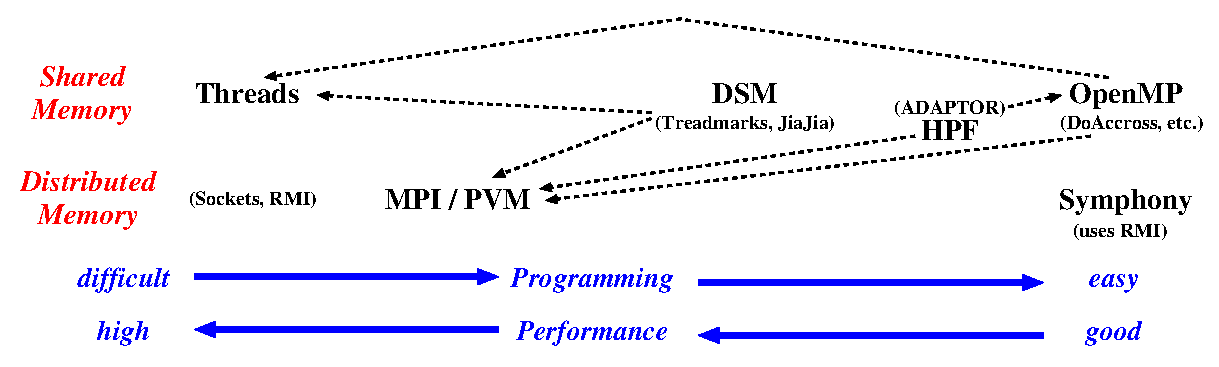
\includegraphics[width=\textwidth]{Figures/ParallelSoftware.eps}
    \caption{Possible software models to be used for parallel programming. 
      For a description of the used abbreviations see table \ref{tab:ParallelAbbrev}.
      Difficult/Easy programming refers to the time needed to implement
      parallel algorithms using a certain model.}
    \label{fig:ParallelSoftware}
  \end{center}
\end{figure}
\begin{table}[htbp]
  \begin{center}
    \begin{tabular}{ll}
      DSM & Distributed Shared Memory \\
      HPF & High Performance Fortran \\
      MPI & Message Passing Interface \\
      PVM & Parallel Virtual Machine \\
      RMI & Remote Method Invocation \\
      OpenMP & Open Multiple Processes \\
    \end{tabular}
    \caption{Abbreviations used for the models in parallel programming.}
    \label{tab:ParallelAbbrev}
  \end{center}
\end{table}

But what are the differences between the software models?
\subsubsection{OpenMP}
If you want to spend
less time for coding, you should use OpenMP, a directives based approach;
You just have to insert comments (FORTRAN) or pragmas (C/C++) before the 
code you want to be executed in parallel.
The DoAccross directives and other directives based models were the
forerunners of OpenMP and should not be used anymore. The advantage of OpenMP is,
that you do not have to change your serial program, you just add comments
(or pragmas in C/C++) and most of the work is done by an appropiate compiler.
The drawbacks are the restriction to shared memory machines\footnote{There are
meanwhile software packages available, which convert OpenMP programs into 
usual Fortran/C/C++ code using MPI calls and therefore running on
distributed memory machines, e.g. OdinMP, etc.}
and the worse performance compared to good MPI programs.

\subsubsection{Symphony}
An alternative to OpenMP would be to use a kind of server, which distributes
small pieces (jobs) of your problem to many machines available and collects
the results to be processed later on, therefore exploiting a kind of distributed memory
model, but with no communication between the different jobs.
An example of this philosophy
realized in Java is a project developed at the University of Freiburg called
Symphony (see later on). 

\subsubsection{HPF}
If you want to spend more time thinking about how the data and the 
work can be distributed to the avialable processors, then you can go with 
HPF. HPF employs a data distributed model and 
is of course only available to Fortran 77/90/95 programmers and
have not found a very widespread use. But still it is a viable tool for
many problems and it is available on almost any computer architecture.
An interesting solution is the (free) ADAPTOR software, which converts HPF programs
to Fortran 90 with MPI calls or you can convert to OpenMP directives. 

\subsubsection{MPI / PVM}
Even more work and time has to be spent to write a MPI/PVM program. PVM was
the first available message passing interface, but has meanwhile been
abandoned by most people in favour of MPI, which is today the standard to use
for writing message passing programs. 

In this model you have to 
take care of everything yourself. You have to tell the computer, when, what and 
with who you want to exchange messages (data). This works by writing a single
program, which consists of several calls to MPI functions\footnote{You just have
to add a library to your compiler commands and you have to use a special program
to run the parallel MPI program (mpirun).}. There are functions for
sending messages from one CPU to another or you can send data from one CPU to
all other CPUs working on the same problem (a so called communicator).
The compiler (or to be  exact the library) just translates the MPI commands
to a lower level of networking commands, depending on the available library and
network hardware used. 

For example if you have a ethernet network with
several PCs running Linux/Windows, you can install a free version of MPI
(e.g. MPICH or LAM) and compile the MPI programs. The code will then be run on all
requested CPUs using the ethernet protocol to communicate and exchange data.
On a shared memory machine (including SMP machines) 
you can also use MPI, but this time the communication could
be done directly, so using MPI for an SMP machine is usually a big overhead
and should be avoided. The biggest advantage of MPI is, that it is available
for all platforms and hardware architectures, so it is completly portable.

\subsubsection{(Java) Threads}
The last alternative for writing parallel programs is using threads. Threads are small
parts of a single program, which are to be executed by the same CPU using
time sharing or by a separate CPU. 
So it is kind of using MPI calls, but this time you have to use functions,
which are implemented on the level of the underlying operating system.
This means your program is very fast in starting a job on a different CPU
and it is very easy to have global variables, but you are confined to
shared memory machines and to a certain operating system. So this is usually
not the model of choice for a scientific problem. 

But with Java this is
not (always) correct anymore. In Java it is very easy to use threads and
because Java is portable across all platforms, almost all of 
the restrictions just mentioned no longer apply. 
But of course you still have to work a bit more to get a threaded
program running correctly compared to an MPI or OpenMP program. But it 
definitly has become an interesting alternative, if Java is becoming much
faster in the next few years (and we are sure it will).

\subsubsection{Amdahl's Law}
At last we want to mention an important point, which has already been made 
by G. Amdahl in 1967: If you denote the part of a program to be run
sequentially by $f$, then the ``speedup'' $S_N$ can be calculated as
$$ S_N =\frac{T_1}{T_N} = \frac{N}{1+f(N-1)} .$$
Where the speedup is defined as the ratio of the time to complete 
the serial program and the time needed by using $N$ processors simultaneously. 
\begin{figure}[htbp]
  \begin{center}
    \includegraphics[angle=-90,width=\textwidth]{Figures/Amdahl.eps}
    \caption{Amdahls law with some examples for the value of the serial
      part $f$ of a program.}
    \label{fig:Amdahl}
  \end{center}
\end{figure}
This dramatically restricts the performance gained by using many CPUs.
So the sequential parts of a parallel program should be kept as small
as possible. Fortunately the speedup depends on the problem size and
will increase for bigger problems. 

%%%%%%%%%%%%%
\subsection{The Ehrenfest Model using a Parallel Program}

Here we want to demonstrate, how to write and use a parallel program
employing the Ehrenfest model as an example problem. 

\subsubsection{Symphony}
Using Symphony is very easy in this case. The idea is to compute the same
model (number of time steps) with different number of fleas on dog one. Then we
can generate very easily the statistics for the Ehrenfest model discussed
in section \ref{sec:EhrenfestModel}.
\inputlisting{Listings_Java/DogFlea.java}
First you have to compile the java program and copy the class file to the directory,
where a  browser can access it 
(e.g. \verb|/home/user/public_html/Symphony/SymphonyTasks| for a unix machine).
Then on the Symphony server machine, which has to have a WWW server 
running\footnote{For example the Apache web server. Apache is freely 
available for all unixes and even for Win32 since a few months ago, 
although the performance is much better on unix.}
you have to edit the file \verb|../Symphony/SymphonyServer/tasks.sym| to
contain the parameters you want to compute, e.g. it could look like this:
{\small
\begin{verbatim}
process=DogFlea;
entryPoint=run;
param(n0d),min=10,max=1000,incr=10;
param(Nd),const=1000;
return (na,nb) as {EVENT @DogFlea @run0};
timeout=1;
\end{verbatim} }
Now you start the Symphony server with 
\begin{verbatim}
  .../Symphony/SymphonyServer/start_server
\end{verbatim}
and on the clients 
(the computers you want to have to participate on the computation)
you start the appletviewer with 
\begin{verbatim}
 appletviewer http://SymphonyServer/~user/Symphony/applet.html ,
\end{verbatim}
where you
have to substitute your Symphony server WWW address and the name of the
user. This assumes you have a unix system, for a Windows system just
change the path accordingly. 

The clients are only computing, if the appletviewer window is visible, so
the user calling the page to start the Symphony applet can decide if she/he
wants to participate or not. On the clients you get the messages:
{\small
\begin{verbatim}
 {DogFlea.59} 
...got to process DogFlea.59
 Results of run; 
 class: DogFlea; 
 entry point: run;  
 Input Field: n0d=810.0;  Input Field: Nd=1000.0; 
 Output Field: na=479;  Output Field: nb=521; 
 Time to process: 3.0 seconds;  
** End of Symphony run **   
\end{verbatim} }
This shows one job, which was run using $810$ fleas initially on dog 1 and
$1000$ fleas alltogether. The results get saved in a file called \verb|event.log|
in a directory 
\begin{verbatim}
 .../Symphony/SymphonyServer/data/DogFlea/run0/ 
\end{verbatim}
The second step is to extract the results from the logfile, e.g. use the
follwowing program:
\inputlisting{Listings_Java/ConvertSymphony.java}
This produces a data file containing the variables (\verb|n0d Nd na nb|) 
and can be plotted using Ptplot or by any plotting program e.g. gnuplot (after 
starting gnuplot use for example \verb|gnuplot "gnu.out" using 1:3|).

%%%%%%%%%%%%%%%%%%%%%%%

\subsubsection{Java Threads}
Now we take a look at Java Threads, the details can be found in
\cite[]{JavaThreads}. 

A \emph{thread} is a shorthand for ``thread of control'' and stands for a
section of code executed independendly of other threads in a single program.
You are actually already familiar with this concept, because every operating
system today uses multitasking to run multiple programs at the same time sharing
one CPU. If you view these ``tasks'' as single threads, we only have to
extend to multiple threads in a singl program. In Java the JVM is responsible
of starting multiple threads in your code. That is also where the restrictions
come in: most of the JVMs did not support multiple threads running in
parallel on SMP machines, meaning that you do not have real parallel 
programs working with all available CPUs. Nevertheless is the concept
of threads useful for single processor machines. For example we have 
already met this case in the last chapters, where we did extensive
calculations, while still the user had the opportunity to interrupt the 
calculation by hitting a mouse button or moving the mouse. This is only
possible, if during the simulation a thread is always asking for user 
intervention. The JVM thread implementation of multiple threads, but only one thread
being active at a time, is called \emph{green threads}\footnote{These
threads are user-level threads. It means that the first thread started by the
operating system starts multiple threads itself and the operating system
does not interfere. These are also called lightweight processes, because
the kernel of the operating system does not have to do much work for
switching from one user-level thread to another}. All JDK 
implementations employ these green threads for Java threads.

\begin{figure}[htbp]
  \begin{center}
    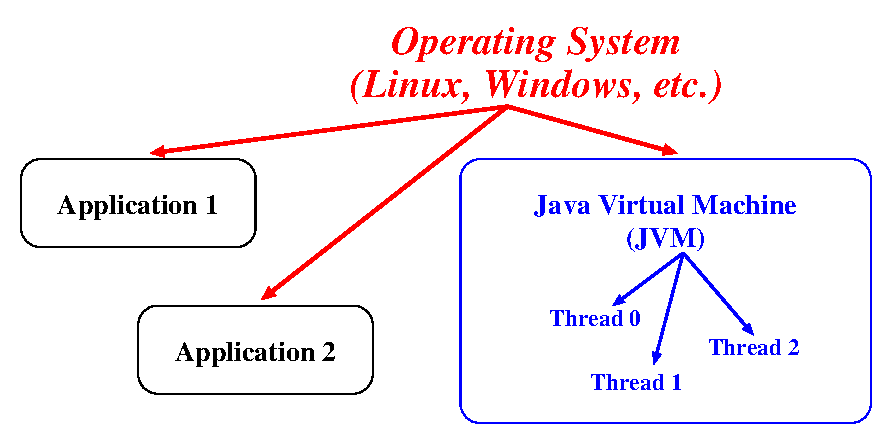
\includegraphics[width=\textwidth]{Figures/Threads.eps}
    \caption{A multitasking operating system employing a Java Virtual Machine, which runs multiple threads.}
    \label{fig:Threads}
  \end{center}
\end{figure}

Here we want to concentrate on running different threads on several CPUs.
To that end we need a JVM, which supports ``real'' threads or so-called
native threads\footnote{These are so-called kernel-level threads. This time the
kernel of the operating system has to do some context switching and
therefore there is a little overhead compared to user-level threads.}. 
If your JVM supports native threads should be stated in the documentation
somewhere. For the JDK, all the 1.2 versions on all platforms support and
use native threads without further notification. For JDK 1.1.7 running
Linux/Solaris you can get an additional package, which supports native
threads. To call the native threads version you have to use
\verb|java -native Program|.

Native threads are only useful for threads, which do some heavy calculations.
For the case where you only want to have user interaction and calculation
running in ``parallel'', like in the molecular dynamics simulation or the
Ising model, we are better off with the green threads. 

Applets also employ threading, but here we also have to check if we
``only'' have green threads or even have native threads available.
Actually I do not know of any JVM implemented in a web browser capable
of using native threads yet. But the need for threads in applets is even
more important, because if you have an applet on top of a web page and
the applet has to do some time consuming initializations, it will stop
showing the rest of the page until the applet finishes. If the browser
itself uses a seperate thread for the applet, this is not a concern, but
still you should use threads for time consuming operations in an applet.

Now let us take a look at our example and how we can use Java threads to
speed up our calculation of the Ehrenfest model. The Thread class in Java
is located in the \verb|java.lang| package. We basically have two 
ways of defining a thread before we can use it. 
\begin{itemize}
\item Extending the thread class in a separate file. Example:
First the thread:
\begin{small}
\begin{verbatim}
   public class OurOwnThread extemds Thread {       
       public void run() {
            // here we can do computations
       }
   }
\end{verbatim}
\end{small}
and second the calling class:
\begin{small}
\begin{verbatim}
   public class OurOwnThread1 {
      public static void main(String[] args) {
         // main method of application
         OurOwnThread own = new OurOwnThread();
         own.start();  // this calls the run() method of the thread
      }
   }       
\end{verbatim} 
\end{small}
\item Implementing a runnable interface. Implementing an interface means
  to supply all necessary methods needed for an interface (here the thread)
  to be build up. For a thread you only have to supply the \verb|run()| method,
  nothing else. Example:
\begin{small}
\begin{verbatim}
   public class OurOwnThread2 implements Runnable {
      public static void main(String[] args) {
         // main method of application
         OurOwnThread2 own = new OurOwnThread2();
         Thread th = new Thread();
         th.start();  // this calls the run() method of the thread
      }
      public void run() {
         // the computation method of the thread
      }
   }       
\end{verbatim}
\end{small}
\end{itemize}
Which way you use does not matter and there is no preferred way, it just
depends on your personal preference.

Now there might be a little confusion about the \verb|start()| method.
There is a \verb|start()| method in the Applet class and one in the Thread
class. The same applies to the \verb|stop()| method. So you have to be a little 
bit careful to which method you refer, but it will always be clear from
the context. And a second remark is about the \verb|run()| method. 
You should never call directly, but always call the  \verb|start()| method
of the thread, which in turn starts the thread and calls the \verb|run()| method.
This is a common mistake, because the program starts and works correct, but
it does start the threads sequentially and not in parallel. 

Now finally let us see how we can apply this to our problem. First we need
the thread:
\lstinputlisting{Listings_Java/DogFleaCalc.java}
And second we need a ``server'', which starts the threads and collects
the answers; this is very similar to the Symphony example and will be
the same in the MPI problem:
\lstinputlisting{Listings_Java/DogFleaThreads.java}
The \verb|void join()| method returns only, if the thread is marked
as no longer being alive and therefore being completed. The join method
also accepts an argument, which is the timeout (a long variable) in milliseconds.
 If you give
a timeout, join returns at the latest after the timeout time.

If you compile both classes and start the \verb|DogFleaThreads.java| class
you will see the threads starting and stopping, here we always start two
threads at a time and wait for both to finish. 

Try the two different executions:
\begin{itemize}
\item \verb|java -green DogFleaThreads|
\item \verb|java -native DogFleaThreads|
\end{itemize}
On UNIX you can use the \verb|time| command to check the execution times.
Here we run both commands (\verb|-green| on the left and \verb|-native| on the right)
on a Linux machine using the JDK1.2 on a single
and a two processor machine.

On a single processor machine you get:
\begin{multicols}{2}
\begin{small}
\begin{verbatim}
 Waiting !
at time s=0:  0
at time s=100000:  499
at time s=0:  333
at time s=100000:  496
 Ready !
 Waiting !
at time s=0:  666
at time s=100000:  475
at time s=0:  999
at time s=100000:  530
 Ready !
 
real    4m32.880s
user    4m1.290s   <-----------
sys     0m4.750s   <-----------
at time s=0:  0
at time s=0:  333
 Waiting !
at time s=100000:  515
at time s=100000:  512
 Ready !
at time s=0:  666
 Waiting !
at time s=0:  999
at time s=100000:  476
at time s=100000:  489
 Ready !
 
real    4m25.449s
user    4m2.110s    <----------
sys     0m6.300s    <----------
\end{verbatim} 
\end{small}
\end{multicols}
And on a 2 processor machine you will get:
\begin{multicols}{2}
\begin{small}
\begin{verbatim}
 Waiting !
at time s=0:  0
at time s=100000:  491
at time s=0:  333
at time s=100000:  496
 Ready !
 Waiting !
at time s=0:  666
at time s=100000:  473
at time s=0:  999
at time s=100000:  478
 Ready !

real    0m14.397s      <-----------
user    0m12.610s
sys     0m0.180s
at time s=0:  0
at time s=0:  333
 Waiting !
at time s=100000:  481
at time s=100000:  518
 Ready !
at time s=0:  666
 Waiting !
at time s=0:  999
at time s=100000:  503
at time s=100000:  472
 Ready !

real    0m8.216s         <------------
user    0m12.970s
sys     0m0.170s
\end{verbatim} 
\end{small}
\end{multicols}
Neglect the absolute times given, because we used two totally different 
machines for the tests. But look at the relative timings comparing
the native and the green threads on single and multiple processor machines.

By using a 2 processor machine we almost get a speedup of 2 for this problem
(look at the real time),
and on the single processor machine the performance gets worse by using
native threads (look at the user and system time), which is due 
to the nature of kernel-level threads and
user-level threads. The use of JDK1.2 is just due to the fact that a JIT is 
already supplied with the 1.2 version and we wanted to speed up the program.
You could also use another JIT with JDK1.1.

You should also note that the messages appear randomly and do not in
any order. So if you use output in threads you should always remember,
that there is no given order for the output to be send to the screen. This
will be also true for MPI programs.

The reason for the randomness is the way of the JVM to execute the threads.
This is called the ``Scheduling of threads''. Like the operating
system has to tell, which processes are to be executed at what time
and how long the JVM has to use a scheduling algorithm to tell each
thread, when it has to go on and when it has to wait. Because this
is a difficult isu, we do not go into details. The scheduling used
in the JDK is not written in detail in the JVM specifications and therefore their
are certain differences on different platforms. It states only that it
has to be an pre-emptive, priority based scheduler, where the priority
(greater equal to zero) is a natural number and the highest number
refers to higher priority. Threads of equal priority are the case, which
makes most of the problems. For a more detailed discussion and examples
of e.g. a Round-Robin Scheduler written in Java,
you should take a look at a book about threading (like \cite[]{JavaThreads}).
 
Just to complete this section, we want to mention some more methods of
the Thread class. 
\begin{description}
\item[static void sleep(long t)] This method stops the execution of a 
  thread for \verb|t| milliseconds.
\item[boolean isAlive()] Another useful method is the \verb|isAlive()| method, which 
returns true, if the thread is still ``running''. Do not confuse this
with  the \verb|boolean isActive()| method of the Applet class, which
returns true, if the applet is somewhere still executing (executing
code between the \verb|start()| and the \verb|stop()| method.).
\item[static Thread currentThread()] This returns the thread object of the current
  thread
\item[static int activeCount()] Returns how many thread are running.
\end{description}
There are many other methods, but many of them are depreciated as of
Java 2 (e.g. \verb|suspend(), stop(), resume(),| etc.), 
because they introduce serious problems.

There is one last remark you should keep in mind: Never restart a thread!! 
The reason for this is a bit involved and the interested reader should
refer to \cite[]{JavaThreads}.

%%%%%%%%%%%%%%%%%%%%%%%%%%%5
\subsubsection{MPI and Java}

??????????? which interface ???


%%%%%%%%%%%%%%%%%%%%%%%%%%%%%%%%%%%%%%%%%%%%%%%%%%%%%%%%%%%%%%%%

\section{Master equations, entropy, asnd the $H$--theorem}
In this section we are going to discuss in more detail the connections between
the master equation and the entropy. In particular we want to derive the
$H$--theorem, which we have already mentioned in the previous section. 
The starting point of our discussion will be a master equation of the general
form
\begin{equation}
\label{eq:MasterH}
  \frac{\partial}{\partial t} P(x,t) = \sum_{x'} 
   [w(x|x') P(x',t) - w(x'|x) P(x,t)]
\end{equation}
and we want to discuss separately two cases: (i) the transition matrix is
symmetric, i.e.,
\begin{displaymath}
  w(x|x') = w(x'|x);
\end{displaymath}
(ii) the condition of detailed balance is satisfied
\begin{equation}
\label{eq:MasterDetBal}
  w(x|x') P_{\textrm{eq}}(x',t) = w(x'|x) P_{\textrm{eq}}(x,t).
\end{equation}

\subsection{Case (i): The symmetric transition matrix}
It is evident that for these case the master equation (\ref{eq:MasterH}) can
be written in the simplified form
\begin{equation}
\label{eq:MasterHSym}
  \frac{\partial}{\partial t} P(x,t) = \sum_{x'} 
   w(x|x') [P(x',t) - P(x,t)].
\end{equation}
Thus, at equilibrium we have
\begin{displaymath}
  \frac{d}{dt}P = 0,
\end{displaymath}
since $w(x|x') \ge 0$. Hence,
\begin{equation}
\label{eq:MasterHEqSym}
  P_{\textrm{eq}} (x,t) = \textrm{const} = \frac{1}{\Omega},
\end{equation}
where 
\begin{displaymath}
  \Omega = \sum_x 1.
\end{displaymath}

In order to demonstrate that equilibrium is approached in a unique way we
choose the following $H$--function
\begin{displaymath}
  H(t) = \sum_x P(x,t) \ln P(x,t).
\end{displaymath}
We now calculate explicitely the time derivative of the above defined
function. For notational ease we replace the sum by an integral. We find
\begin{displaymath}
  \frac{d}{dt} H(t)  = \int dx 
\left[ \left( \frac{\partial}{\partial t} P(x,t) \right) \ln P(x,t) +
         \frac{\partial}{\partial t} \ln P(x,t) 
     \right].
\end{displaymath}
Because of the conservation of the norm of the probability density
\begin{displaymath}
  \int dx P(x,t) = 1,
\end{displaymath}
the time derivative of the $H$--function is
\begin{displaymath}
  \frac{d}{dt} H(t)  =  \int dx  
         \left( \frac{\partial}{\partial t} P(x,t) \right) \ln P(x,t).
\end{displaymath}
Now, we insert the master equation (\ref{eq:MasterHSym}) into the above
expression and obtain
\begin{eqnarray*}
 \frac{d}{dt} H(t) & = & \int dx \int dx' w(x|x') 
                            \left( P(x',t) - P(x,t) \right) 
                                \ln P(x,t), \\
                   & = & \int dx \int dx' w(x'|x) 
                            \left( P(x,t) - P(x',t) \right) 
                                \ln P(x',t).
\end{eqnarray*}
The second line in the above expression has been obatined by changing the
names of the integration variables. Exploiting the symmetry of the transition
matrix,  the time derivative of the $H$--function 
can be written in the symmetrized  form
\begin{displaymath}
  \frac{d}{dt} H(t) = \frac{1}{2}  \int dx \int dx' w(x'|x) 
             \left( P(x',t) - P(x,t) \right) 
             \left( \ln P(x,t) -  \ln P(x',t) \right).  
\end{displaymath}
Recalling that
\begin{displaymath}
  (a -b) (\ln a  \ln b) \ge 0 
\end{displaymath}
for $a$, $b >0$ it follows for the time derivative of the $H$--function that
\begin{displaymath}
   \frac{d}{dt} H(t) \le 0.
\end{displaymath}
The $H$--function decreases monotonically as a function of time during the
time evolution of the Matkov process. The $H$--function gets stationary when
the condition
\begin{displaymath}
  P(x,t) \rightarrow P_{\textrm{eq}} (x); \;\;\; 
           P_{\textrm{eq}}(x) =P_{\textrm{eq}}(x') 
\end{displaymath}
is satisfied for each pair of states $x$ and $x'$, which are connected by
nonvanishing transition matrix elements. If the set of the states $x$ does not
decay into two or more independent subsets, the equilibrium is uniquely
characterized by the form (\ref{eq:MasterHEqSym}).

\subsubsection{Case (ii): Detailed balance}
Case (ii) is of course more general than case (i). In order to
investigate this second case we choose the following $H$--function
\begin{equation}
\label{eq:MasterHDetBal}
  H(t) = \int dx p(x,t) \ln \frac{P(x,t)}{P_{\textrm{eq}}(x)}
\end{equation}
and show that again the $H$--theorem holds, i.e.,
\begin{displaymath}
  \frac{d}{dt} H(t) \le 0.
\end{displaymath}
To this end we define a new matrix, say
\begin{equation}
\label{eq:MasterWbar}
  \bar{w}(x|x') = w(x|x') P_{\textrm{eq}}(x'),
\end{equation}
which becasue of the property of detailed balance (\ref{eq:MasterDetBal}) 
is symmetric.  With the help of the definition (\ref{eq:MasterWbar}) we can
write the master equation in the form 
\begin{displaymath}
  \frac{\partial}{\partial t} P(x,t) = \int dx'  \bar{w}(x'|x)
   \left[ \frac{P(x',t)}{P_{\textrm{eq}}(x')} -
          \frac{P(x,t)}{P_{\textrm{eq}}(x)}         \right].
\end{displaymath}
Inserting this form of the master equation in the definition of the
$H$--function (\ref{eq:MasterHDetBal}) we can show in a form analgous to the
previous subsection
\begin{eqnarray*}
  \frac{d}{dt} H(t) & = & \frac{1}{2} \int dx \int dx' 
                   \bar{w}(x'|x) \left[ \frac{P(x',t)}{P_{\textrm{eq}}(x')} -
          \frac{P(x,t)}{P_{\textrm{eq}}(x)}         \right]
            \left( \ln \frac{P(x,t)}{P_{\textrm{eq}}(x)} 
               - \ln \frac{P(x',t)}{P_{\textrm{eq}}(x')}  \right), \\
    & \le & 0.
\end{eqnarray*}
If the system is ergodic, after some time it reaches the equlibrium
\begin{displaymath}
  P(x,t) \longrightarrow P_{\textrm{eq}}(x) 
\end{displaymath}
and the $H$--function assumes its minimal value. the $H$--function 
(\ref{eq:MasterHDetBal}) has two important properties. 
The special form of
the $H$--function allows the proof of a $H$--theorem also for the Boltzmann
equation. The interesting point is taht the Boltzmann equation itself being a
nonlinear equation for the distribution in a 6 dimensional one--partice
phase space is not a master equation. However, the linareised Boltzmann
equation is a master equation.

The function $H$ is an addtitive quantity. Consider two independent systems
with states $x$ and $y$ and probability densities $p(x)$ and $q(y)$. We regard
the two systems as a combined system with states $(x,y)$ and probability
density $p(x)q(y)$. Then the $H$--functional of the combined system is the sum
of the $H$--functionals of the two subsystems
\begin{displaymath}
  \int dx \int dy P(x) Q(y) \ln \frac{P(x) Q(y)}
                                     {P_{\textrm{eq}}(x) Q_{\textrm{eq}}(x)}=
\int dx P(x)  \ln \frac{P(x)}{P_{\textrm{eq}}(x)}  +
\int dx Q(x)  \ln \frac{Q(x)}{Q_{\textrm{eq}}(x)}.
\end{displaymath}
Thus, $H$ is an exstensive quantity.
 
Because of these two important properties one could like  to  identify $H$
with the entropy
of the second Hauptsatz of thermodynamics. However, it is important to keep in
mind, that the $H$--functional we introduced is a functional of a
nonequilibrium distribution, whereas the the thermodynamic entropy is defined
for a  system at equilibrium. The nonequilibrium $H$ functional allows 
therefore a  generalization of the thermodynamic entropy
\begin{displaymath}
  S = -k H + S^{\textrm{eq}},
\end{displaymath}
where $k$ is Boltzmann's constant and $S^{\textrm{eq}}$ is a constant term,
which is independent of $p(x)$. At equilibrium $H=0$, so that 
$S^{\textrm{eq}}$ is the thermodynamic entropy.


\section{Nonequilbrium thermodynamics}
\subsection{balance equations of fluid dynamics}
In classical theoretical physics the dynamics of fluids is described with the
help of the balance equations of nonequlibrium thermodynamics for the mass,
the momentum, and the energy. These balance equations are derived under the
assumption, that in a small volume element of the bulk of the fluid mass,
momentum, and energy are in a local thermal equilibrium. Evidently, if one
considers the molecular structure of a fluid, one has to regard the mass, the
momentum, and the energy density as mean value of stongly fluctuating
microscopic quantities. These fluctuations are neglected in the purely
macroscopic classical description. 

However, as we have seen in the preceeding sections, fluctuations play a
fundamental role in systems out or approaching equilibrium. Typical situations
in which fluctuations are of central importance in the description of fluids
occur near equilibrium in the form of small Gaussian fluctuations in the
macroscopic variables, these are the so--called hydrodynamic fluctuations,
and the large non--Gaussian fluctuations in the velocity filed of turbulent 
fluids.

For these reasons it seems natural to look for a  stochastic, mesoscopic
formulation of fluid dynamics. On this macroscopic level we will have the same
numbero f variables as in the macroscopic level of description. The dynamics
of theses variables will no longer be deterministic but stochastic. The
mesocopic approach should satisfy four conditions:

(i) In the limit of vanishing fluctuations the equation of motion for the 
mean values of the stochastic variables
should be identical with the balance equations of fluid dynamics.

(ii) In a linear noise approximation we should obtain from the master equation
defining the stochastic process the linear Langevin equation of fluctuating
hydrodynamics. In this way nonequlibrium thermodynmics should be contained in
the approach. 

(iii) In the continuum limit the characteristci function of the stochastic
process should generate the complete hierarchy of coupled equations for the
moments of the velocity fileds, which are known from the theory of
turbulence. In this way the master equation should describe correctly the the
turbulent, non--Gaussian fluctuations. 

(iv) The mesoscopic formulation should lead to simple and efficient numerical
alghorithms, which should be vectrorizable and parlalleizable.

In the  following we are going to investigate such a formulation for a very
simple balance equation, the one dimensional Burgers equation, which is the
equation of motion for a one--dimensinal velocity field $v(x,t)$,

The Burgers equation is a one--dimensional version of the navier--Stokes
equation. It is often used in gas dynamics since it shows shock wave
solutions, and as a simple model of turbulence.

\subsection{The definition of the phas space}
In this subsection we define the space of
states of the fluid. Once the accessible states of the fluid
are known it
is possible to construct a master equation governing the
probabilistic
time evolution of the system. 

The first step of the construction of an appropriate phase space
consists
in the division of physical space into a number of cells
centered at the points $x_{\lambda}$ which we
label by an integer--valued index $\lambda \in {\bf{Z}}$.
For the purpose of
general (three dimensional)
considerations it suffices to use cubic cells of size $\delta l^{3}$;
in practice, shape and size of the cells can be adapted to
the confining geometry of the flow. Here the
cells are
just one--dimensional intervals of length $\delta l$ since we are
considering
one space dimensional examples only. Depending on the physical
situation under study the number of cells may be finite or
infinite. In
the stochastic simulation this number is, of course, always finite
and
fluids of (practically) infinite size have to be modelled by
imposing suitable
boundary conditions.

we now
interpret the
velocity field $u(x,t)$ appearing in the Navier--Stokes equation
as an expectation value of a discrete stochastic process
$N_u^{\lambda}(t) \in {\bf{Z}}$, i.~e. we define
\begin{equation}
\label{EXPEC}
u(x_{\lambda},t) =
\delta u \;\; \langle N_u^{\lambda}(t) \rangle \;\;\; .
\end{equation}
The above equation provides the connection between the macroscopic
and the stochastic description of fluid motion. Within
the stochastic
description the velocity is a time--dependent random variable
$N_u^{\lambda}$,
i.~e. a stochastic process governed by a master equation to be
defined below.
On the other hand, the velocity on a macroscopic scale,
that is on the scale
accessible to standard experimental observation, is given by an
expectation
value, and therefore obeys the deterministic Navier--Stokes
equation.
The velocity unit $\delta u$ has been introduced in order to obtain
a discrete stochastic process $N_u^{\lambda}$. Thus it represents
the size
of the smallest possible changes of the state of the fluid
in the discretized
phase space. This means that within our description a positive value
$\delta u \cdot N_u^{\lambda}$ of
the random velocity in the cell ${\lambda}$ can be intepreted as
the presence
of $N_u^{\lambda}$ velocity particles each carrying the velocity
$\delta u$.
Correspondingly, a negative value $\delta u \cdot N_u^{\lambda}$
is to be
interpreted as the presence of $\mid N_u^{\lambda} \mid $
antiparticles of
velocity. Defining the positive and negative part of
$N_u^{\lambda}$ as
\begin{equation}
N_{u+}^{\lambda} := \left\{ \begin{array}{lll}
       N_u^{\lambda} \;\; &,&  \;\;\; N_u^{\lambda} \geq 0 \\
                            0 \;\; &,& \;\;\; N_u^{\lambda} < 0
                            \end{array}
                            \right. \;\;\; , \;\;\;
N_{u-}^{\lambda} := \left\{ \begin{array}{lll}
               0 \;\; &,&  \;\;\; N_u^{\lambda} \geq 0 \\
               N_u^{\lambda} \;\; &,& \;\;\; N_u^{\lambda} < 0
                            \end{array}
                            \right. \;\;\; ,
\end{equation}
we write:
\begin{equation}
N_u^{\lambda} = N_{u+}^{\lambda} + N_{u-}^{\lambda} \;\;\; .
\end{equation}
Thus we see that within our description the mesoscopic
state of the fluid may be viewed as a many velocity particle state
and is completely fixed by specifying
the number $N_u^{\lambda}$ of velocity particles in each cell
$\lambda$.
Formally, the resulting phase space may be written as
\begin{equation}
\label{PHASESPACE}
\Gamma = \left\{ \left( N_u^{\lambda} \right)_{\lambda \in {\bf{Z}}}
         \mid N_u^{\lambda} \in {\bf{Z}}
\right\} \;\;\; .
\end{equation}

\subsection{The construction of the master equation}

In order to obtain the master equation for the Burgers model  we proceed
as follows: We show explicitly how stochastic processes can be
constructed whose expectation values obey the corresponding
terms in the Burgers equation equation. These stochastic processes
are defined by a master equation which is a time evolution equation
for the joint probability distribution $P=P(N_u^{\lambda};t)$ in the
phase space $\Gamma$. From this probability distribution the
expectation
value for an arbitrary observable ${\cal{O}}$ may be evaluated
according to
\begin{equation}
\langle {\cal{O}} \rangle = \sum_{\left\{ N_u^{\lambda} \right\}}
{\cal{O}} \, P \left( \{ N_u^{\lambda} \} ;t \right) \;\;\; .
\end{equation}

\subsubsection{Viscosity as a many--particle random walk}
In this section we are going to describe viscous fluids within
our stochastic
approach. In the simplest cases, the Navier--Stokes equation
containing only
viscous forces reads
\begin{equation}
\label{NVSDIFF}
\frac{\partial u}{\partial t} =
   \frac{1}{R} \frac{\partial^2 u}{\partial x^2} \;\;\; .
\end{equation}
As in the preceeding section we want to define a stochastic process
$N_u^{\lambda}(t)$
in such a way that its expectation value
\begin{equation}            \label{EXP2}
u(x_{\lambda},t) = \delta u \; \langle N_u^{\lambda}(t) \rangle
\end{equation}
obeys the diffusion--like equation (\ref{NVSDIFF}).

It is well--known that the probability distribution
$\phi_{\lambda}(t)$, $\lambda \in {\bf{Z}}$,
of a one particle
random walk fulfills in the continuous limit a
diffusion equation. More precisely, let us consider a continuous
time
random walk in one dimension. The probability distribution
$\phi_{\lambda}(t)$ obeys the following master equation
\begin{equation}
\label{RDMWALK}
\frac{\partial \phi_{\lambda}}{\partial t} =
  d \cdot \left(
\phi_{\lambda+1} -2 \phi_{\lambda} + \phi_{\lambda-1}
 \right) \;\;\; , \;\;\; d=\mbox{const.} \;\;\; .
\end{equation}
It is easy to see from the above equation that in the limit
of infinitesimal
small random steps,
\begin{equation}
\phi_{\lambda}(t) \longrightarrow \phi(x=\delta l \cdot \lambda,t)
\;\;\; ,
\end{equation}
the probability distribution $\phi(x,t)$ is a solution of the
diffusion
equation
\begin{equation}
\label{DIFF1}
\frac{\partial \phi}{\partial t} = D
\frac{\partial^{2} \phi}{\partial x^{2}} \;\;\; , \;\;\; 
D:= {\lim}_{\delta l \rightarrow 0} \left( \delta l^2 \; d \right)
\;\;\; .
\end{equation}

The formal analogy of the diffusion equation (\ref{DIFF1}) with
the one
dimensional Navier--Stokes equation (\ref{NVSDIFF}) is obvious.
However, there is a fundamental difference between these two
equations.
The diffusion equation (\ref{DIFF1}) describes the time
evolution of a
{\em probability distribution} which is normalized and positive
definite.
In contrast, the one dimensional Navier--Stokes equation
(\ref{NVSDIFF})
is an equation for an {\em expectation value} which might be
negative and not
normalizable. Thus, the stochastic process
underlying (\ref{NVSDIFF}) can {\em not} be described by a
{\em one particle}
random walk.
Therefore, one has to leave the one particle picture. To this end,
we consider
a collection of independent velocity particles each of which is
governed by
Eq. (\ref{RDMWALK}). The state of the resulting collective system
\cite{KAMPEN} is characterized by the set of numbers $N_u^{\lambda}$
of velocity particles in all cells $\lambda$.
Thus, in this many--particle picture one disregards the identity of
the
individual particles and is merely interested in the occupation
numbers
$N_u^{\lambda}$ of particles in each cell.
(Note, that in the one--particle
picture the state of the system is completely specified by giving
the
location $\lambda$ of the particle.)

In the framework of the many particle picture the one--particle
density
$\phi_{\lambda}(t)$ is replaced by the many particle probability
distribution $P(N_u^{\lambda};t)$. The master equation defining the
time evolution of $P(N_u^{\lambda};t)$ can be obtained from the
one--particle master equation by multiplying the one--particle
transition rates
with the occupation number $N_u^{\lambda}$ of cell $\lambda$,
\begin{eqnarray*}
\frac{\partial P}{\partial t} & = &    \frac{1}{R \, \delta l^2}
                                    \sum_{\lambda} \left(
          (N_{\lambda} +1) P(\ldots,N_{\lambda-1}-1, N_{\lambda}+1, \ldots) 
        + (N_{\lambda} +1) P(\ldots, N_{\lambda}+1, N_{\lambda+1} -1, \ldots) 
                                      \right. \\
                            && - \left. \right).
\end{eqnarray*}
Introducing the shift--operators ${\bf E}_{\lambda}$ which operate on an
arbitrary function $F$ of the random varoables as 
\begin{eqnarray}
{\bf{E}}_{\lambda} F(\ldots, N_u^{\lambda}, \ldots)  & = &
 F(\ldots, N_u^{\lambda} + 1, \ldots)                   \nonumber \\
{\bf{E}}_{\lambda}^{-1} F(\ldots, N_u^{\lambda}, \ldots) & = &
 F(\ldots, N_u^{\lambda} - 1, \ldots)  \;\;\; ,
\end{eqnarray}
we can write the master equation as
\begin{equation}
\label{DIFFME}
\frac{\partial P}{\partial t} =    \frac{1}{R \, \delta l^2}
\sum_{\lambda} \left[ \left( {\bf{E}}_{\lambda -1}^{-1}
     {\bf{E}}_{\lambda}
     - {\bf{1}} \right) N_u^{\lambda}
     + \left( {\bf{E}}_{\lambda +1}^{-1} {\bf{E}}_{\lambda}
     - {\bf{1}} \right) N_u^{\lambda} \right] P  \;\;\; ,
\end{equation}
where $\delta l$ denotes the cell size.
Since the expectation value of $N_u^{\lambda}$ is a statistical
guess of the
one--particle density at the point $\lambda$
the velocity field (\ref{EXP2})
obeys the diffusion equation (\ref{NVSDIFF}) as required.
Until now we implicitly restricted our attention to the collective
random walk of positive velocity particles. Obviously, to be
consistent
with our general picture of particles and antiparticles of velocity
we have to generalize the master equation describing viscous fluids
in order
to allow for the correct treatment of antiparticles of velocity.
Since a one--particle jump to the right is equivalent to a
one--antiparticle
jump to the left and vice versa, the master equation (\ref{DIFFME})
has to
be modified in the following way: In order to describe the
diffusion of
antiparticles the numbers $N_u^{\lambda} = N_{u-}^{\lambda}$
are replaced
by their absolute values $\mid N_u^{\lambda} \mid =
- N_{u-}^{\lambda}$
and the shift operators 
${\bf{E}}_{\lambda \pm 1}^{-1} {\bf{E}}_{\lambda}$ by
${\bf{E}}_{\lambda \pm 1} {\bf{E}}_{\lambda}^{-1}$.
Consequently, if both particles and antiparticles of velocity
are present
the master equation can be written:

\begin{eqnarray}
\label{DIFFOP}
\frac{\partial P}{\partial t} &=&  \frac{1}{R \, \delta l^2}
\sum_{\lambda} \left[ \left( {\bf{E}}_{\lambda -1}^{-1}
{\bf{E}}_{\lambda}
     - {\bf{1}} \right) N_{u+}^{\lambda}
     + \left( {\bf{E}}_{\lambda +1}^{-1} {\bf{E}}_{\lambda}
     - {\bf{1}} \right) N_{u+}^{\lambda} \right] P  \nonumber \\
 && - \frac{1}{R \, \delta l^2}
 \sum_{\lambda} \left[
      \left( {\bf{E}}_{\lambda -1} {\bf{E}}_{\lambda}^{-1}
     - {\bf{1}} \right)  N_{u-}^{\lambda} 
     + \left( {\bf{E}}_{\lambda +1} {\bf{E}}_{\lambda}^{-1}
     - {\bf{1}} \right) N_{u-}^{\lambda} \right] P  \nonumber \\
&=:&  {\cal{A}}_d \, P \;\;\; ,
\end{eqnarray}
where we introduced the ``diffusion operator'' ${\cal{A}}_d$.

Having presented the master equation defining the time evolution
of the stochastic process $\left\{ N_{\lambda} \right\}$ we now
demonstrate that
our requirement explained in subsection x is satisfied, i.e.,
we show that
the expectation value of the stochastic process
$\delta u \langle N_{\lambda} \rangle$ indeed
obeys a discrete form of the Burgesr equation containg only viscous forces.. 

More generally, let us first derive an appropriate form for the time
evolution equation of the expectation value of an arbitrary function
${\cal{F}} \left( \{ N_{\lambda} \} \right)$ of the stochastic
variables.
To this end, we consider an expression of the form
$\langle {\bf{E}}_{\lambda + 1}^{-1}
{\bf{E}}_{\lambda} {\cal{F}} \rangle$.
Recalling that the expectation
value involves a multiple sum over all integers
$N_{\lambda}$ it is easy
to show with the help of the definition of the operators
${\bf{E}}^{\pm}_{\lambda}$, Eq.~(\ref{SHIFT}), and by shifting
the summation indices appropriately that the following equation
holds
\begin{equation}         \label{PROP1}
\langle {\bf{E}}_{\lambda +1}^{-1} {\bf{E}}_{\lambda}
{\cal{F}} \rangle
= \langle {\cal{F}} \rangle \;\;\; .
\end{equation}
This equation is true, of course, for any other product of
shift operators
appearing in our master equation (\ref{MASTEREQ}).
Thus, these products of shift operators when
acting on a function of the stochastic variables have no influence
on its expectation value and can, within the angular brackets,
always be replaced by the identity. Since the time evolution
operator
${\cal{A}}$ contains the above products of shift operators
only in the
form $({\bf{E}} {\bf{E}} - {\bf{1}})$, Eq.~(\ref{PROP1})
implies that
\begin{equation}
\label{AFEXPEC}
\langle {\cal{A}} \; {\cal{F}} \rangle =
\sum_{\left\{N_{\lambda} \right\}}
{\cal{A}}\; {\cal{F}} P = 0
\;\;\; .
\end{equation}
Introducing the commutator (the function ${\cal{F}}$ being
regarded as a
multiplication operator)
\begin{equation}
\left[ {\cal{F}}, {\cal{A}} \right] := {\cal{F A}} - {\cal{A \; F}}
\end{equation}
and exploiting relation~(\ref{AFEXPEC}) equation~(\ref{TIMEEV})
takes the form
\begin{equation}     \label{HGLN}
\frac{\partial}{\partial t} \langle {\cal{F}} \rangle = \left\langle
\left[ {\cal{F}} , {\cal{A}} \right] \right\rangle
\;\;\; .
\end{equation}
Thus, the time derivative of the expectation value of a function
${\cal{F}}$ of the stochastic variables is equal to the expectation
value of the commutator $\left[{\cal{F}},{\cal{A}}\right]$.
For the special case of the first moments of the stochastic process
$\delta u N_{\lambda}$ we have
\begin{equation}
\label{MOMENT2}
\delta u \frac{\partial}{\partial t} \langle N_{\lambda} \rangle
= \delta u \; \left\langle \left[ N_{\lambda} , {\cal{A}} \right]
\right\rangle
\;\;\; .
\end{equation}
In order to determine the commutator $[N_{\lambda}, {\cal{A}}]$ we
proceed by evaluating some useful the commutators.
Let us begin with the calculation of the commutator $[N_s, {\bf E}_{s'}]$ by
looking at how it operators on an arbitrary function of the stochastic
variables. Let us consider first the case that $s=s'$. We have
\begin{eqnarray*}
  [N_s,{\bf E}_s] F(\ldots, N_{s}, \ldots) & = & 
         N_s {\bf E}_s F(\ldots, N_{s}, \ldots) -
    {\bf E}_s  N_s F(\ldots, N_{\lambda}, \ldots) \\
                    & = & N_s  F(\ldots, N_{s} +1 , \ldots)
                         - (N_s +1) F(\ldots, N_{s} +1 , \ldots) \\
                    & = & - {\bf E}_s  F(\ldots, N_{s}, \ldots).
\end{eqnarray*}
For the case that $s \ne s'$ the calculation is similar
\begin{eqnarray*}
   [N_s,{\bf E}_{s'}] F(\ldots, N_{s}, \ldots) & = & 
      N_s {\bf E}_{s'} F(\ldots, N_{s}, \ldots)
             -
    {\bf E}_{s'}  N_s F(\ldots, N_{\lambda}, \ldots) \\
   &&    N_s F(\ldots, N_{s}, N_{s'}+1, \ldots) - 
            N_s F(\ldots, N_{s}, N_{s'}+1, \ldots) \\
      & = & 0.    
\end{eqnarray*}
Summarizing, we can write
\begin{displaymath}
  [N_s,{\bf E}_{s'}] = - {\bf E}_s \delta_{s,s'}.  
\end{displaymath}
Similarly, we can show that
\begin{displaymath}
   [N_s,{\bf E}_{s'}^{-1}] = {\bf E}_s^{-1} \delta_{s,s'}. 
\end{displaymath}
Another useful commutator is
\begin{eqnarray*}
  [N_s, {\bf E}^{-1}_{s' \pm 1} {\bf E}_{s'}] & = &
        [N_s, {\bf E}^{-1}_{s' \pm 1}] {\bf E}_{s'}
         +{\bf E}^{-1}_{s' \pm 1} [N_s, {\bf E}_{s'}] \\
     & = & {\bf E}^{-1}_{s' \pm 1} {\bf E}_{s'} \delta_{s' \pm 1,s} 
             - {\bf E}^{-1}_{s' \pm 1} {\bf E}_{s'}  \delta_{s',s} \\
     & = & {\bf E}^{-1}_{s' \pm 1} {\bf E}_{s'} 
                      (\delta_{s' \pm 1,s} -\delta_{s',s} ). 
\end{eqnarray*}
In order to determine the equation of motion for the expecation value of 
random velocity variable we thus have to compute first the commutator
$[N_{\lambda},{\cal{A}}_d]$. We obtain 
\begin{eqnarray*}
[N_{\lambda},{\cal{A}}_d] &=&  \frac{1}{R \delta l^2} \sum_{s'}
                  \left[ [N_s,{\bf E}^{-1}_{s' - 1}{\bf E}_{s'}]
                              (N_{s'}^+ - N_{s'-1}^-)    \right. \\
               && + \left. [N_s,{\bf E}^{-1}_{s' + 1}{\bf E}_{s'}]
                        (N_{s'}^+ - N_{s'+1}^-)   \right]  \\
              & = &   \frac{1}{R \delta l^2} \sum_{s'}
                \left[ {\bf E}^{-1}_{s' + 1}{\bf E}_{s'} 
                        (\delta_{s'-1,s} - \delta_{s',s})  
                        (N_{s'}^+ -  N_{s'-1}^-)
                        \right. \\
                   && + \left. {\bf E}^{-1}_{s' + 1}{\bf E}_{s'}
                          (\delta_{s'+1,s} - \delta_{s',s})  
                         (N_{s'}^+ - N_{s'+1}^-)    \right]  \\
             & = & \frac{1}{R \delta l^2} 
                   \left\{  {\bf E}^{-1}_{s}{\bf E}_{s+1}
                           (N_{s+1}^+ -  N_{s}^-) 
                           - {\bf E}^{-1}_{s-1}{\bf E}_{s}
                           (N_{s}^+ -  N_{s-1}^-) 
                                \right. \\
            && +   \left.  {\bf E}^{-1}_{s}{\bf E}_{s-1}
                           (N_{s-1}^+ -  N_{s}^-)  
                        - {\bf E}^{-1}_{s+1}{\bf E}_{s}
                           (N_{s}^+ -  N_{s+1}^-)       \right\}.
\end{eqnarray*}
Before taking the expecation value of the above expression we have to notice
that wheneever in the sum $\sum_{\{ N_{ \lambda \} }}$ the shift operators appear
on the extreme left they can be replaced by 1. This is easy to show with the
help of the definition of the shift operators and by shifting  appropriately
the summation indices.
With the help of this trick it is evident that we have
\begin{equation}
\label{MOMENT3}
\delta u \; \frac{\partial}{\partial t}
\langle N_{\lambda} \rangle  = 
\nu \frac{\delta u}{ \delta l^2}
  \langle N_{\lambda +1}^+ - 2 N_{\lambda}^+ + N_{\lambda -1}^+ +
          N_{\lambda +1}^- - 2 N_{\lambda}^- + N_{\lambda -1}^-
          \rangle .
\end{equation}
Recalling that $N_{\lambda} = N_{\lambda}^+ + N_{\lambda}^-$ the
time evolution equation of the first moment of the stochastic
process
$N_{\lambda}$ can be written as
\begin{equation}
\label{MOMENT4}
\delta u \; \frac{\partial}{\partial t} \langle N_{\lambda}
\rangle =
\nu \frac{\delta u}{\delta l^2}
  \langle N_{\lambda +1} - 2 N_{\lambda} + N_{\lambda -1} \rangle
   \;\;\; .
\end{equation}
Since, the equation is linear in $N_{\lambda}$ we have, of course,
$v_{\lambda} = \delta u \langle N_{\lambda} \rangle$ and hence
we immediately obtain a discretized version of the Burgers equation without
convective terms. 
\begin{equation}
\label{DISCRETEBURGERS}
\frac{\partial}{\partial t} v_{\lambda}(t) =
\nu \frac{v_{\lambda +1} -2 v_{\lambda} +
v_{\lambda -1}}{\delta l^2}
- \frac{1}{2} \frac{v_{\lambda+1}^2 -
v_{\lambda -1}^2}{2 \; \delta l }
\;\;\; ,
\end{equation}
which, in turn, leads to Burgers' equation~(\ref{BURGERS}) in the
continuum limit $\delta l \longrightarrow 0$.

\subsubsection{The nonlinear convection term}
Up to now, we have shown how to deal with  viscous diffusion. 
However, it is of great importance
to include
within the stochastic theory nonlinear interactions which, for
example, enter
the Navier--Stokes equation through the nonlinear inertial term
$(\vec{u} \cdot \vec{\nabla}) \vec{u}$. It is a remarkable fact
that interpreting
the inertial term as a nonlinear convection term a
stochastic interpretation
in terms of one--particle jumps can be found. As will be shown
here, again,
the many--particle picture is absolutely necessary.

As before we are looking for the stochastic process
$N_u^{\lambda}(t)$
the expectation value of which obeys Burgers' equation. Obviously,
the
stochastic process underlying the
nonlinear convection term is fundamentally different from the
previously
introduced stochastic processes: It is not a random walk of
a collection
of independent particles.
The construction of the Hydrostochastic form of the
convection term will now be given heuristically
within the many particle picture.
 

Let us consider what happens in a specific cell $\lambda$ occupied
by
$N_u^{\lambda} \geq 0$ velocity particles. Within the stochastic
approach
convection may be modelled as a jump process from cell
$\lambda$ to cell $(\lambda + 1)$.
Thus, the stochastic process is
completely specified by giving the transition rates for
these elementary jumps. The probability for the jump of a
{\em{specific}} particle situated in cell $\lambda$ is proportional
to the velocity at $\lambda$ and, hence, proportional to the
number of velocity particles in cell $\lambda$.
Consequently, the
{\em total} transition rate is proportional to the number of pairs
of velocity particles in the cell $\lambda$, i.~e. to
$N_u^{\lambda} \cdot
(N_u^{\lambda} - 1) / 2$. On dimensional grounds the
proportionality factor
is found to be $\delta u / \delta l$ (note that transition rates
have
the dimension of an inverse time) and we obtain the following master
equation for the convection of velocity particles:
\begin{equation}
\frac{\partial P}{\partial t}  = 
\frac{\delta u}{\delta l} \sum_{\lambda}
     \left( {\bf E}_{\lambda +1}^{-1} {\bf E}_{\lambda} - {\bf 1}
    \right) \frac{1}{2} N_u^{\lambda} (N_u^{\lambda}-1) P
\;\;\; .
\end{equation}
 

It can be shown that the above form of the master equation
for the convection term
leads to a discretization of the differential operator
$u\partial /\partial x$ which is of order $\delta l$. In order to
obtain a discretization of this differential operator which is of
order $\delta l^{2}$ the following symmetrized
form of the master equation will be used:
\begin{eqnarray}
\label{TRANSPORT1}
\frac{\partial P}{\partial t} & = & \frac{1}{2}
\frac{\delta u}{\delta l} \left\{
                          \sum_{\lambda}
     \left( {\bf E}_{\lambda +1}^{-1} {\bf E}_{\lambda} - {\bf 1}
    \right) \frac{1}{2} N_u^{\lambda} (N_u^{\lambda}-1) P \right.
               \nonumber \\
& &  + \left.  \sum_{\lambda}
       \left( {\bf E}_{\lambda}^{-1} {\bf E}_{\lambda -1} - {\bf 1}
    \right) \frac{1}{2} N_u^{\lambda} (N_u^{\lambda}-1) P \right\}
               \nonumber \\
&=:&  {\cal{A}}_c \, P          \;\;\; ,
\end{eqnarray}
where we abbreviated the effect of the
right hand side by defining the ``convection operator''
${\cal{A}}_c$.

Constructing Eq.~(\ref{TRANSPORT1}) we assumed that
$N_u^{\lambda} \geq 0$.
The general master equation describing both the presence
of velocity particles
and antiparticles can now easily be derived.
Let us assume, that cell $\lambda$ contains
$\mid N_u^{\lambda}\mid = - N_{u-}^{\lambda}$
antiparticles of velocity. The elementary jumps of the antiparticles
can be obtained from those of the particles of velocity by simply
reversing
the directions of the jumps, i.~e. all antiparticles jump to
the left.
However, since the process of an antiparticle jumping to the left is
identical to the process of a particle jumping to the right, the
above master
equation describes the combined convection of particles and
antiparticles
of velocity if $N_u^{\lambda}$ is replaced by
$\mid N_u^{\lambda} \mid$.

Summarizing the master equation of the Burgers model reads
\begin{eqnarray}
\label{BURGERSMEQ}
\frac{\partial P}{\partial t} &=&
\left\{ {\cal{A}}_d + {\cal{A}}_c \right\} P
                \nonumber \\
& =  &  \frac{1}{R \, \delta l^2}
\sum_{\lambda} \left[ \left( {\bf{E}}_{\lambda -1}^{-1}
{\bf{E}}_{\lambda}
     - {\bf{1}} \right) N_{u+}^{\lambda}
     + \left( {\bf{E}}_{\lambda +1}^{-1} {\bf{E}}_{\lambda}
     - {\bf{1}} \right) N_{u+}^{\lambda} \right] P  \nonumber \\
 &&  - \frac{1}{R \, \delta l^2}
 \sum_{\lambda} \left[
      \left( {\bf{E}}_{\lambda -1} {\bf{E}}_{\lambda}^{-1}
     - {\bf{1}} \right)  N_{u-}^{\lambda} 
     + \left( {\bf{E}}_{\lambda +1} {\bf{E}}_{\lambda}^{-1}
     - {\bf{1}} \right)  N_{u-}^{\lambda}  \right] P  \nonumber \\
&  & + \frac{1}{2}
\frac{\delta u}{\delta l} \left\{
                          \sum_{\lambda}
    \left( {\bf E}_{\lambda +1}^{-1} {\bf E}_{\lambda} - {\bf 1}
          \right) \frac{1}{2} \mid N_u^{\lambda}\mid
          (\mid N_u^{\lambda} \mid -1) P \right.
               \nonumber \\
& & + \left.  \sum_{\lambda}
       \left( {\bf E}_{\lambda}^{-1} {\bf E}_{\lambda -1} - {\bf 1}
          \right) \frac{1}{2} \mid N_u^{\lambda}\mid
           (\mid N_u^{\lambda}\mid -1) P \right\}
           \;\;\; .
\end{eqnarray}
Let us now demonstrate how the macroscopic equation may be derived from the
above equation. To this end we have only to compute the commutator 
$[N_{\lambda},{\cal{A}}_c]$ with the help of (??)
\begin{eqnarray*}
  [N_s, {\cal{A}}_c] & = & \frac{\delta u}{4 \delta l} \sum_{s'}
                        [N_s, {\bf E}_{s'+1}^{-1} {\bf E}_{s'}]
                          (N_{s'}^2 + N_{s' +1}^2) \\
                     & = & \frac{\delta u}{4 \delta l} \sum_{s'}
                     {\bf E}_{s'+1}^{-1} {\bf E}_{s'}
                       (\delta_{s'+1,s} - \delta{s',s}) 
                       (N_{s'}^2 + N_{s'+1}^2) \\
                    & = &  \frac{\delta u}{4 \delta l} \left\{
                      {\bf E}_{s}^{-1} {\bf E}_{s-1}
                       (N_{s-1}^2 + N_{s}^2)
               +      {\bf E}_{s+1}^{-1} {\bf E}_{s}
                           (N_{s}^2 + N_{s+1}^2)   \right\}.
\end{eqnarray*}
for sufficiently small $\delta u $ the number of velocity
particles $N_u^{\lambda}$ becomes large one expects that
fluctuations are
small and, therefore, that the approximation
\begin{equation}
\langle \left( N_u^{\lambda} \right)^2 \rangle \approx
\langle N_u^{\lambda} \rangle^2
\end{equation}
holds to a sufficient degree of accuracy.
Eq.~(\ref{COMMUT}) may then be
written as an equation for $u_{\lambda}$,
\begin{equation}
\frac{\partial u_{\lambda}}{\partial t} +
\frac{1}{2} \frac{u_{\lambda +1}^2 -
u_{\lambda -1}^2}{2\delta l} =
\frac{1}{R} \frac{u_{\lambda +1} -2u_{\lambda}
+ u_{\lambda -1}}{\delta l^2} \;\;\; .
\end{equation}
Obviously, this equation is nothing but the discretized
version of the
Burgers equation~(\ref{BURGERS}) which emerges in the continuum
limit
$\delta l \longrightarrow 0$.
In deriving the above macroscopic equation for the expectation value
$u_{\lambda}$ we neglected, of course, all higher moments of
the stochastic
process $N_u^{\lambda}$. As is well--known the above master
equation,
defining a nonlinear stochastic process, leads to an infinite
dimensional
system of coupled differential equations for the moments. Thus,
in order to
derive more rigorously from our master equation
the macroscopic equation and to investigate the
dynamics and influence of fluctuations one has to
employ a more systematic
method. Such a method is provided by the well--known
$\Omega$--expansion~\cite{KAMPEN}. Applying this
expansion to the master
equations of Hydrostochastics reveals that, in fact,
the macroscopic
equations are equivalent to the equations of fluid dynamics.
Furthermore,
it can be shown that within the linear noise approximation the
fluctuations
superimposed on the macroscopic dynamics can be identified with
those
fluctuations derived from the theory of fluctuating
hydrodynamics~\cite{LANDAU}.
Thus, the stochastic dynamics implied by our master equation
formulation
can, indeed, be given a clear physical interpretation as we will see in one of
the next setions.

\subsection{The stochastic simulation algorithm}
It is the aim of this section to show that the master equation formulation
of the Burgers equation naturally leads to very transparent numerical
simulation algorithms.
Basically, the stochastic simulation method generates an ensemble of
realizations of the stochastic process $\{ N_{\lambda} \}$.
From this ensemble
the physical quantities of interest, e.~g. the mean velocity field
and correlation functions,
can then be evaluated as ensemble averages.
The stochastic simulation algorithm consists of 3 basic steps:

{\bf{1.}} Let us assume that at time $t$ the state of the system is given
by $\{ N_{\lambda}(t) \}$. In the first step, the time $t+\tau$ of the
next transition is determined. Our algorithm uses a stochastic time step
$\tau$ to be evaluated as follows.
Obviously, the total transition rate
$W(\left\{ N_{\lambda}(t) \right\}) $ is  given by
\begin{equation}
W(\left\{ N_{\lambda} \right\}) =
\sum_{\lambda =0}^{M} w_{\lambda} =
\sum_{\lambda =0}^M \left(
\frac{2 \nu}{\delta l^2}
\mid N_{\lambda} \mid
+ \frac{1}{2} \frac{\delta u}{\delta l} 
N_{\lambda}^2  \right) \;\;\; ,
\end{equation}
where $w_{\lambda}$ denotes the rate for those transitions in which
$N_{\lambda}$ is changed.
Consequently, the probability 
for the next transition to occur somewhere in the system
within the infinitesimal time step $d\tau$ is
$W(\left\{ N_{\lambda}(t) \right\}) d\tau$.
The total transition rate $W$ determines the waiting time distribution,
i.~e. the probability distribution of the time $\tau$ the system remains in the
state $\left\{N_{\lambda}(t)\right\}$. In the stochastic simulation
the random number $\tau$ which determines the time for the
next transition to occur can be obtained by the inversion method
with the help of the following formula
\begin{equation}
\tau = - \frac{1}{W(N^{\lambda}(t))} \ln \eta \;\;\; ,
\end{equation}
where $\eta$ is a uniformly distributed random number on the interval
$[0,1]$.

{\bf{2.}} Having determined the transition time we have to perform a specific
transition, i.e. we have to determine the new state
$\{ N_{\lambda}(t+\tau ) \}$ of the system. To this end, one chooses
according to the relative probabilities
$w_{\lambda}/W$ a certain cell.
Once a definite cell $\lambda$, say, has been chosen the new state of the
system is to be selected from the following possibilities:  \\
1. Diffusive transitions:
\begin{displaymath}
\left. \begin{array}{lcl}
       N_{\lambda} & \rightarrow & N_{\lambda} - s \\
       N_{\lambda + 1} & \rightarrow & N_{\lambda + 1} + s
       \end{array} \right\}
\mbox{probability} = \frac{\nu}{\delta l^2}
            \frac{\mid N_{\lambda} \mid}{w_{\lambda}}
\end{displaymath}
\begin{displaymath}
\left. \begin{array}{lcl}
       N_{\lambda} & \rightarrow & N_{\lambda} - s \\
       N_{\lambda - 1} & \rightarrow & N_{\lambda - 1} + s
       \end{array} \right\}
\mbox{probability} = \frac{\nu}{\delta l^2}
    \frac{\mid N_{\lambda} \mid}{w_{\lambda}}
\end{displaymath}
where
\begin{displaymath}
s = \left\{ \begin{array}{rcll}
           +1 & \hspace{1cm}, & \mbox{for} & N_{\lambda} \ge 0 \\
           -1 & \hspace{1cm}, & \mbox{for} & N_{\lambda} < 0
           \end{array}
           \right. \;\;\; .
\end{displaymath}

2. Convective transition:
\begin{displaymath}
\left. \begin{array}{lcl}
       N_{\lambda} & \rightarrow & N_{\lambda} - 1 \\
       N_{\lambda + 1} & \rightarrow & N_{\lambda + 1} + 1 
       \end{array} \right\}
    \mbox{probability} = \frac{\delta u}{4\delta l}
    \frac{N_{\lambda}^2 + N_{\lambda+1}^2}{w_{\lambda}}
\end{displaymath}
Note that each of these transitions corresponds to one of the 5
terms in our master equation~(\ref{MASTEREQ}) and that the 
transition probabilities given above add up to 1.
Performing one of these transitions yields the new state
$\left\{ N_{\lambda}(t+\tau) \right\}$.

{\bf{3.}} The complete trajectory of the stochastic process can
be determined by repeating the above scheme until a desired final time
is reached. Finally, by generating a large number $S$
of realizations of the stochastic process $\left\{ N_{\lambda}(t) \right\}^j$,
$j=1, \ldots , S,$ one can evaluate the interesting quantities as
ensemble averages.

{\bf{3.}} The complete trajectory of the stochastic process can
be determined by repeating the above scheme until a desired final time
is reached. Finally, by generating a large number $S$
of realizations of the stochastic process $\left\{ N_{\lambda}(t) \right\}^j$,
$j=1, \ldots , S,$ one can evaluate the interesting quantities as
ensemble averages.

The simplicity of the above scheme makes clear that the numerical 
simulation of a stochastic process defined by our multivariate master equation
is straightforward. In the following we shall exemplify this by showing
some stochastic simulations of shock wave solutions of Burgers equation.

Originally Burgers proposed the equation (\ref{BURGERS})
as a simple one--dimensional model of homogeneous turbulence. The
main
features of the Navier--Stokes equations are retained in the above
equation.
The nonlinearity has the same structure as in the Navier--Stokes
equation,
and the dissipative term is also of the same type.  Only the
pressure term
is missing, so that one has to expect a relaxation of turbulence
with time.
The model also lacks an equation of continuity, so that it
describes in
practice a one--dimensional compressible flow. The Burgers equation
is
particularly appealing because the analytical solutions of the
initial value
problem is known \cite{WHITHAM}. These solutions represent,
for example, nonlinear wave solutions like shock waves and ``humps''.
Thus, Burgers' equation is interesting as it makes possible the study
of
the interplay of nonlinear propagation and viscous diffusion.
\subsubsection{Shock waves}
The first example we are going to treat is the shock wave
solution of Burgers'
equation. The shock wave solution is obtained for the following
initial
condition 
\begin{equation}                                             \label{INITSH}
u(x,0) = u_0(x) = \left\{ \begin{array}{rcl}
                        1 & , \;\;\; x < 0 \\
                        0 & , \;\;\; x > 0
                        \end{array} \right. \;\;\; .
\end{equation}
The diffusion and the convection of this initial step are described
by the following time--dependent solution
\begin{equation}
\label{SHOCK}
u(x,t) =
\frac{1}{1+h(x,t) \exp \left[ R \left( x-t/2 \right) /2 \right] }
\;\;\; ,
\end{equation}
where the function $h(x,t)$ is defined by
\begin{equation}
h(x,t) = \frac{ \mbox{erfc} \left( -\sqrt{R/4t} \: x \right)}
   {\mbox{erfc} \left( \sqrt{R/4t} \: \left( x-t \right) \right)}
              \;\;\; .
\end{equation}
The function $\mbox{erfc}(x)$ is known as the conjugated error
function, and
is given by
\begin{equation}
\mbox{erfc}(x) = \frac{2}{\sqrt{\pi}} \int_x^{\infty} dy \;
                   \exp \left(-y^2 \right) \;\;\; .
\end{equation}


As a first example, we depict in Fig.~1 a stochastic simulation of a shock
wave for the Reynolds number $R \equiv \nu^{-1}=100$
which develops from the step function initial condition
\begin{equation}
\label{INIT1}
v(x,0) = \left\{ \begin{array}{cc}
                 1 \;\;\;, & x<0  \\
                 0 \;\;\;, & x>0
                 \end{array} \right. \;\;\; .
\end{equation}
This initial condition corresponds to the initial configuration
of the stochastic variables $\left\{N_{\lambda}\right\}$ given by
\begin{equation}
\label{INIT2}
N_{\lambda}(0) = \left\{ \begin{array}{rc}
                 \mbox{int}(1/\delta u) \;\;\;, & \lambda < 0  \\
                 0 \;\;\;, & \lambda>0
                 \end{array} \right. \;\;\; .
\end{equation}
In Fig.~1 the exact analytical solution of Burgers' equation is represented
by the lines, whereas the symbols mark the results of the simulation.
Fig.~2 shows a simulation obtained for the same initial condition and the same
numerical parameters; however, the Reynolds number was set equal to
infinity, i.~e. $\nu = 0$. This figure clearly demonstrates the great stability
of the stochastic simulation algorithm. 

As a final example we depict in Fig.~3 the simulation of the
confluence of two shocks propagating with different velocities to the right
($R=100$). Again the analytical solution for this problem \cite{WHITHAM}
is indicated by the lines.

\section{Hydrodynamic fluctuations}
In section 2 we proposed a master equation for the stochastic
description of Burgers' equation. This master equation
has been constructed in such a way that the
expectation value of the stochastic process  (\ref{EXPEC}) obeys
in the limit $\delta u \longrightarrow 0$, i.~e. in the limit of
large numbers $N_{\lambda}$, a discretized version of Burgers' equation.
By some stochastic simulations we demonstrated in Section 3 that
this yields a simple numerical approach to fluid dynamical
computations. Of course, the stochastic description by a master equation
implies fluctuations around the macroscopic value of the
velocity field governed by Burgers' equation.

In this section we present a systematic analysis of the stochastic
process $N_{\lambda}$. This analysis proves that, in fact, the macroscopic
equation pertaining to $N_{\lambda}$ is nothing but Burgers' equation.
Furthermore, it is shown that the fluctuations around the macroscopic
velocity which are predicted by our master equation,
are those expected from the theory of hydrodynamic fluctuations.
The basic tool of the following analysis will be the
well--known van Kampen's $\Omega$--expansion \cite{KAMPEN}. Basically, this
method is a consistent expansion of the master equation in powers of
a small quantity $\Omega^{-1}$ which has to be identified from the
physical parameters of the model under study.
The first step in our analysis is, thus, to identify the appropriate small
quantity in our master equation which allows for an $\Omega$--expansion.
Recall that the construction of the master equation was based on the equation
\begin{equation}
v(x_{\lambda},t) = \delta u \langle N_{\lambda} \rangle \;\;\; .
\end{equation}
This equation connects the stochastic process $N_{\lambda}$ to the mean
velocity $v(x_{\lambda},t)$ which obeys Burgers' equation.
It follows from this equation that $\delta u^{-1}$ is approximately proportional
to $N_{\lambda}$. Since in the limit
of infinitely large numbers $N_{\lambda}$ one expects a well--defined macroscopic
law to emerge from the mesoscopic formulation
the quantity $\delta u$ turns out to be an appropriate
small parameter for the $\Omega$--expansion, i.e., in the following
we study the limit
\begin{equation}                                  \label{LIMIT}
\Omega^{-1} = \delta u \longrightarrow 0 \;\;\;   .
\end{equation}
Assuming that the fluctuations of $N_{\lambda}$ are small
it is natural to split the stochastic process $\delta u N_{\lambda}$ into two
parts: the first part is a macroscopic variable $v_{\lambda}$ which satisfies
a deterministic evolution equation, whereas the second part
$w_{\lambda}=\delta u^{1/2} \eta_{\lambda}$ describes the small stochastic
deviations from this deterministic time evolution:
\begin{equation}
\label{ANS}
\delta u N_{\lambda} = v_{\lambda} + \delta u^{1/2} \eta_{\lambda}
\equiv v_{\lambda} + w_{\lambda}
\;\;\; .
\end{equation}
In this equation $v_{\lambda}$ is introduced as an intensive quantity which
is independent of $\delta u$. Also, the new stochastic variable
$\eta_{\lambda}$ is assumed to be independent of
$\delta u$ to leading order. This means that equation~(\ref{ANS})
expresses the expectation that the fluctuations $w_{\lambda}$
around the macroscopic values
are proportional to $\delta u^{1/2}$.

We are now in the position to perform the $\Omega$-expansion along
the lines given by van Kampen. Since the new stochastic variables are
$\eta_{\lambda}$ we first introduce the transformed
probability distribution $\Pi$
\begin{equation}                                     \label{PI}
P\left( \left\{N_{\lambda} \right\};t \right) =
 \delta u^{-(M+1)/2}
   \Pi \left( \left\{ \eta_{\lambda} \right\};t \right)
\end{equation}
for which we have
\begin{equation}
\frac{\partial P}{\partial t} = \frac{\partial \Pi}{\partial t}
          +\sum_{\lambda} \frac{\partial \Pi}{\partial {\eta}_{\lambda}}
                          \frac{d {\eta}_{\lambda}}{dt} 
= \frac{\partial \Pi}{\partial t} -\delta u^{-1/2}
          \sum_{\lambda} \frac{\partial \Pi}{\partial {\eta}_{\lambda}}
                          \frac{\partial {v}_{\lambda}}{\partial t} 
\;\;\; .
\end{equation}
We also expand the shift operators in powers of $\delta u$:
\begin{equation}
{\bf{E}}_{\lambda}
      = {\bf{1}} + \delta u^{1/2} \frac{\partial}{\partial {\eta}_{\lambda}}
              +\frac{1}{2} \delta u \frac{{\partial}^2}
          {\partial {\eta}^2_{\lambda}} + \cdots \;\;\; .
\end{equation}
Inserting these expressions into the master equation for $\Pi$ and collecting
terms of the same order in $\delta u$ we finally obtain (including terms of 
order $\delta u^0$):
\begin{eqnarray}
\label{OMEGAEX}
\frac{\partial \Pi}{\partial t} &=&
\sqrt{\frac{1}{\delta u}} \sum_{\lambda}
\left\{ \frac{\partial v_{\lambda}}{\partial t} + \frac{1}{2}
        \frac{v_{\lambda +1}^{2} - v_{\lambda -1}^{2}}{2\delta l} -
        \nu \frac{v_{\lambda +1} +
        v_{\lambda -1} - 2v_{\lambda}}{\delta l^{2}}
               \right\}
        \frac{\partial \Pi}{\partial \eta_{\lambda}}
  \nonumber \\
&+& \sum_{\lambda}  -\frac{\partial}{\partial \eta_{\lambda}}
   \left\{
\nu
\frac{\eta_{\lambda +1} + \eta_{\lambda -1} -2 \eta_{\lambda}}{\delta l^2}
- \frac{v_{\lambda +1} \eta_{\lambda +1} - v_{\lambda -1} \eta_{\lambda -1}}
{2 \delta l}  \right\} \Pi  \nonumber \\
&+& \frac{1}{2} \sum_{\lambda \mu} \left\{
D_{\lambda \mu} \frac{\partial^{2}}{\partial\eta_{\lambda}\partial \eta_{\mu}}
\right\} \Pi       \;\;\; .
\end{eqnarray}
Let us explain the meaning of the various terms in this equation.
The first sum is of order $\delta u^{-1/2}$
and, therefore, diverges in the limit $\delta u \longrightarrow 0$ unless
one imposes the condition that the expressions within the curly brackets of
the first sum vanishes for each $\lambda$. In fact, until now the dynamics
of the macroscopic variables $v_{\lambda}$ has not been
specified.
Thus, in order to obtain a well--defined $\Omega$--expansion we now require
that the curly brackets of the first sum vanishes identically. This
condition is easily seen to be equivalent to the requirement that $v_{\lambda}$
obeys the (discretized) Burgers equation (\ref{BURGD}).

The remaining terms of the
master equation for $\Pi$ constitute a linear Fokker--Planck equation
which has
an obvious physical interpretation. The drift term of this Fokker--Planck
equation is
obtained by linearizing Burgers' equation around the
macroscopic solution $v_{\lambda}$. Thus, the drift term governs
the time evolution of small perturbations of the macroscopic variable.

The last term of equation~(\ref{OMEGAEX}) describes a multivariate
diffusion process with diffusion matrix
\begin{equation}     \label{DIFFMAT}
D_{\lambda \mu} :=\left( d_{\lambda} + d_{\lambda -1}  \right)
\delta_{\lambda
\mu} - d_{\lambda} \delta_{\lambda +1, \mu} - d_{\mu} \delta_{\lambda , \mu +1}
\;\;\; ,
\end{equation}
where
\begin{equation}
d_{\lambda} := \nu \frac{{\tilde{v}}_{\lambda} +
{\tilde{v}}_{\lambda + 1}}{\delta l^2}
 + \frac{{\tilde{v}}_{\lambda}^2 + {\tilde{v}}_{\lambda + 1}^2}{4 \delta l}
\;\;\; , \;\;\;\; {\tilde{v}}_{\lambda}:= \delta u
      \langle \mid N_{\lambda} \mid \rangle \;\;\; .
\end{equation}
Since the above Fokker--Planck equation is linear its general solution
represents a nonstationary multivariate
Gaussian process which is completely characterized
by its mean values and variances.
The latter are defined by
\begin{eqnarray}
\langle \eta_{\lambda}(t) \eta_{\mu}(t) \rangle \; &=& \int {\cal{D}} \eta \;
\eta_{\lambda} \eta_{\mu} \;
\Pi \left( \left\{ \eta_{\lambda} \right\};t \right)
        \;\;\; ,
\end{eqnarray}
where
\begin{equation}
{\cal{D}}\eta := d\eta_0 \, d\eta_1 \, d\eta_2 \ldots d\eta_M
\;\;\; .
\end{equation}
It is now straightforward to write down the
dynamic equations for the correlation function
$\langle \eta_{\lambda} \eta_{\mu} \rangle $.
This will be done for the stochastic variables
$w_{\lambda} = \delta u^{1/2}\eta_{\lambda}$
which represent the random velocity fluctuations. Since the equations
of fluctuating hydrodynamics are usually formulated in a continuous
notation we write in the continuum limit
$\delta l \longrightarrow 0$:
\begin{equation}
\langle w_{\lambda}(t) w_{\mu}(t) \rangle \longrightarrow
\langle w(y,t) w(x,t) \rangle   \;\;\; .
\end{equation}
We then obtain from the Fokker--Planck equation (\ref{OMEGAEX})
\begin{eqnarray}
\frac{\partial}{\partial t} \langle w(y,t)w(x,t) \rangle & = &
 \left( \nu \frac{\partial^2}{\partial y^2}
       - \frac{\partial}{\partial y} v(y,t) \right) \langle w(y,t)w(x,t) \rangle
       \nonumber \\
& + & \left( \nu \frac{\partial^2}{\partial x^2}
       - \frac{\partial}{\partial x} v(x,t) \right) \langle w(y,t)w(x,t) \rangle
       \nonumber \\
& + & \delta u \, D_{yx}     \label{wwcorr} \;\;\; ,
\end{eqnarray}
where we introduced the continuum limit of the diffusion matrix
$D_{\lambda \mu}$ as
\begin{equation}
\label{DIFFUSION}
D_{yx} :=  -2 \nu  \frac{\partial}{\partial x} {\tilde{v}}
         \frac{\partial}{\partial x} 
         \delta l \; \delta(y-x)     \;\;\; .
\end{equation}
It should be noted
that the $\Omega$--expansion as presented above is based on the assumption
that the stochastic process $\delta u N_{\lambda}$ 
can be decomposed into a macroscopic part of order
$1$ and a fluctuating part of order $\delta u^{1/2}$. This implies, of course,
that we assume that the solutions of the macroscopic equation are stable.
This condition guarantees that the fluctuations around the macroscopic
variables are bounded~\cite{KAMPEN}.

Let us make an important remark. Our master equation (\ref{MASTEREQ})
describes both the viscous friction and the nonlinear inertial term
of Burgers' equation by stochastic processes. Thus, our stochastic
formulation treats the nonlinear convection term and the dissipative viscosity
term on an equal footing. How\-ever, it is important to note that in the continuum
limit the nonlinear term does not contribute to the fluctuations.
This fact can be clearly seen from the continuum limit (\ref{DIFFUSION})
of the diffusion matrix (\ref{DIFFMAT}).

he above equation for the correlation function $\langle ww \rangle$
now allows to identify the physical meaning of the mesoscopic velocity
and length scales $\delta u$ and $\delta l$ which have been introduced
within our stochastic description. Let us consider the stationary and
spatially homogeneous
velocity fluctuations around a state with constant macroscopic
velocity $v$ and mass density $\rho$.
With these assumptions we obtain  the following stationary
solution (neglecting boundary effects):
\begin{equation}     \label{corrstat}
\langle w(y,t) w(x,t) \rangle_{s} = {\tilde{v}} \delta u \; \delta l \delta (y-x)
\;\;\; . 
\end{equation}
This explicit expression for the velocity
fluctuations enables us to relate the mesoscopic quantities $\delta u$ and
$\delta l$ to thermodynamic state variables. Recall, that the stochastic
process $\delta u N_{\lambda}(t)$ represents, from a microscopic viewpoint,
the average velocity of the real fluid particles of mass $m$ in cell $\lambda$.
We now assume the fluid particles in each cell to be in a local
thermodynamic equilibrium state.
It is then natural to identify the magnitude of the variance of the
random velocity $w$ with the thermodynamic fluctuations $(\Delta u)^2$ of this
average velocity.

From the Maxwell distribution at temperature $T$ we obtain
\begin{equation}
(\Delta u)^{2} = \frac{kT}{\rho \delta l} \;\;\; ,  \label{KT}
\end{equation}
where $k$ denotes Boltzmann's constant. Thus we have
\begin{equation}
\tilde{v} \delta u = \frac{kT}{\rho \delta l}  \;\;\; . \label{FDT}
\end{equation}
Equation~(\ref{FDT}) represents a type of fluctuation--dissipation relation
of our mesoscopic theory.
Note that both mesoscopic parameters, $\delta u$ and $\delta l$, enter
the equation~(\ref{FDT}). Thus, $\delta u$ is fixed once a length scale
$\delta l$ has been chosen. Of course, the magnitude of $\delta l$ is
determined by the very assumptions of local thermodynamic equilibrium which
usually enter non--equilibrium thermodynamics: On the one hand, $\delta l$
has to be chosen in such a way that the number  of fluid particles
contained in a cell is large enough to allow for a reasonable thermodynamic
description. On the other hand, the size of $\delta l$ is limited by the
requirement that the variation of the various quantities over the
cells is small compared to the magnitude of these quantities.

We have seen that the dynamics of the velocity
fluctuations is governed by a linear Fokker--Planck equation.
Of course, the dynamics of the fluctuations can be described as well by
an equivalent Langevin equation.
Invoking our fluctuation--dissipation relation (\ref{FDT})
the Langevin equation for the
stochastic variable $w(x,t)$ reads
\begin{equation}
\label{FH}
\frac{\partial}{\partial t} w(x,t) =
 \left( \nu \frac{\partial^2}{\partial x^2} -
         v \frac{\partial}{\partial x} \right) w(x,t) -
         \frac{\partial}{\partial x} \xi(x,t)
\;\;\; .
\end{equation}
Interpreting $\xi (x,t)$ as the random momentum flux density,
equation~(\ref{FH}) is precisely of the form
of the corresponding equation in fluctuating hydrodynamics (see, for
example,~\cite{GRABERT,FOX}).
The correlation function of the
random momentum flux  can be determined from the diffusion
matrix and our fluctuation--dissipation relation. One finds
\begin{equation}                                 \label{CORRF}
\langle \xi (y,t) \xi (x,t') \rangle = \frac{2kT \nu}{\rho}
              \delta (y-x) \delta (t-t')
\;\;\; .
\end{equation}

Let us sum up what has been achieved in this section. By means of
the simple example of Burgers' equation we have established the connection
of our multivariate master equation description of fluid dynamics to
the theory of fluctuations in fluids. In other words,
the master equation describes both the macroscopic dynamics and the
dynamics of the fluctuations.

\subsection{Couette Flow and Poiseuille Flow}

%%%%%%%%%%%%%%% !!!!!!!!!!!!!!!!!!

\section{Homogeneous turbulence: The Burgers equation}
\subsection{Homogeneous turbulence}
A turbulent fluid is usually characterized by irregular and disordered
temporal variations of the velocity field at each point of the fluid and
conversely  the variations of the velocity vary irregularly from point to
point at a fixed time. Up to now there is no complete quantitative theory of
turbulence, but there are well accepted  qualitative results.

\paragraph{The energy cascade}
The main aspect of the tutbulence problem is the presence in a turbulent fluid
of different length scales. Looking at a turbulent fluid you will notice
vortices with small and large dimensions. For very large Reynolds number there
are very turbulent elements on very large and on very small length scales. The
main role is played be the large vortices, which are of the order of magnitude
of the exterior dimensions of the system under consideration. Lets call thius
legth scale $l$. The order of magnitude of the velocity is of the order of the
variation of the mean velocity $\Delta u$  on the length scale $l$. The large
turbulent elemnetns contain most of the kinetic energy of the turbulent
fluid. Small vortices contain only a small part of the kinetic energy.

The general properties of a given flow are characterized by the Reynolds
number
\begin{displaymath}
  R = \frac{ul}{\nu}.
\end{displaymath}
Abetter characterization is found by introducing Reynolds numbers  for
turbulent elements of different size. Denoting by $\lambda$ the size of the
turbulent element, by $v_{\lambda}$ the order of magnitude of the velocity in
that turbulent element we can define
\begin{displaymath}
  R_{\lambda} \approx \frac{v_{\lambda} \Lambda}{\nu}.
\end{displaymath}
For large values of $R$ also the  the Reynolds numbers $R_{\lambda}$ of the
large vortices ($\lambda \approx l$) are large. Since a large $R$ implies a
small $\nu$, we may follow that t he viscosity does not play a great role  for
the large turbulent elements. Hence it is not to be expected that dissipation
will play a great role for these vortices. Viscosity will affect only the
smallest vortices ($\Lambda_0$), for which $R_{\lambda} \approx 1$. And it is
here that the dissipation takes place. 

The physical picture of what is going on in a turbulent fluid  id due to
L. Richardson (1922). The energy flows from the large vortices into the small
ones. This process occurs without dissipation. The energy flow is disspipated
inthe smallest vortices, where kinetic energy is converted into heat. To make
this process "stationary" it is of course necessary to add energy in the large
length scales. This picture is  called the energy cascade. As we will see, a
major aspect of theis picture is that all quantities involved which belong to
turbulent elements with $\lambda > \lambda_0$ do not depend upon the
viscosity.

\paragraph{The orders of magnitude of the energy dissipation}
The enenergy dissipation is defined as the mean energy which is dissipated pro
time unit and pro mass unit in a turbulent fluid. The order of magnitude of
the energy dissipation may be detremined with the help of quantities which are
characteristic of the large vortices. These quantities are the density of the
fluid $\rho$, the linear dimesnion $l$, and the velocity $\Delta u$. Only a
combination of these 3 quantities has the dimension of a dissipation
$([\epsilon] = J/(kg \cdot s) = m^2 /s^3)$
\begin{displaymath}
  \epsilon \approx \frac{(\Delta u)^3}{l}.
\end{displaymath}
A turbulent flow can be described qualitative as a fluid with a turbulent
viscosity $\nu_{\textrm{turbo}} \neq \nu$. The only dimensionless quantity
with the dimension of aviscosity which may be constructed with the help of 
$\rho$, $\Delta u$, and $l$ is
\begin{displaymath}
  \nu_{\textrm{turbo}} \approx l \Delta u.
\end{displaymath}
We have
\begin{displaymath}
  \frac{\nu_{\textrm{turbo}}}{\nu} \approx R.
\end{displaymath}
Note that $\nu_{\textrm{turbo}}$ gets larger for increasing Reynolds number
$R$. In other words, we can write the energy dissipation also in the form
\begin{displaymath}
  \epsilon \approx \left( \frac{\Delta u}{l} \right)^2 
\end{displaymath}
in accordance with the usual defuinition of viscosity.

\paragraph{The law of Kolmogorow} 
Now we want to look at the properties of the turbulence on the length scale 
$\lambda$, which is assumed to be small with respect to $l$. We look at the
bulk of the fluid and neglect boundary effects. In these domain it is safe to
assume that the turbulence is homogeneous and isotropic. We will now deduce
with the help of similitartity arguments some fundamental results (Kolmogorow,
1941; Obuchow, 1941). The local properties of the turbulence are determined for
$l \gg \lambda \gg \lambda_0$   by $\lambda$, the density $\rho$ and the enegy
diisipation $\epsilon$. The local properties do not depend upon $l$ and
$\Delta u$, which are relevant for the flow as a whole. Furthermore, they do
not depend upon $\nu$. 

The variation of the velocity $v_{\lambda}$ on a length scale $\lambda$ is
easily guessed by considering that the only quantity with the dimension of
avelocity which can be formed with the help of $\rho$, $\epsilon$ and
$\lambda$ is
\begin{equation}
\label{eq:TurboVlambda}
  v_{\lambda} \approx (\epsilon \cdot \lambda)^{1/3}.
\end{equation}
This is the famous law of Kolmogorow andd Obuchow, which states that the
variation of the velocity on a distance of he order $\lambda$ is proporional
to the cubic root of the distance $\lambda$. The velocity $v_{\lambda}$ may be
  regarded as the gelocity of a turbulent element of dimension $\lambda$.

Similarly, the variation of the velocity at a fixed point during the time
$\tau$, which is smaler then characteristic time scale $T \approx l/u$ 
may be estimated by inserting $u\tau$ for $\lambda$ in the above equation 
to be
\begin{equation}
\label{eq:TurboVtau}
  v_{\tau} \approx (\epsilon \cdot \tau \cdot u)^{1/3}
\end{equation}
With the help of 
\begin{displaymath}
  \epsilon \approx \frac{(\Delta u)^3}{l}
\end{displaymath}
Eqs. (\ref{eq:TurboVlambda}) and (\ref{eq:TurboVtau}) 
can be brought in the following suggestive form
\begin{displaymath}
  \frac{v_{\lambda}}{\Delta u} \approx \left( \frac{\lambda}{l}\right)^{1/3}
\end{displaymath}
and, respectively,
\begin{displaymath}
 \frac{v_{\tau}}{\Delta u} \approx \left( \frac{\tau}{T}\right)^{1/3} .
\end{displaymath}
The two above expression make evident the self--similarity property of local
turbulence. The characteristic quantities differ only through the scales in
which the length and the times are measured.

\paragraph{Estimation of the dimensions 
$\lambda_0$ of the smallest turbulent elements}
On the smallest "inner" length scale $lambda_0$ of turbulence the effects of
dissipation are important. The local Reynolds number
we find
\begin{displaymath}
  R_{\lambda} \approx \frac{v_{\lambda}\cdot \lambda}{\nu}
              \approx \frac{\Delta u \cdot \lambda^{4/3}}{\nu l^{1/3}}
              \approx R \left( \frac{\lambda}{l}\right)^{4/3} .
\end{displaymath}
The smallest length scale $\lambda_0$ can be found from the condition that
$R_{\lambda} \approx 1$. We find
\begin{displaymath}
  \lambda_0 \approx \frac{l}{R^{3/4}}.
\end{displaymath}
It is important to notice, that the inner dimesnions of the turbulence gets
rapidly smaller for increasing Reynolds number. This point has to be kept in
mind when performing numerical simulations of the turbulence. For large values
of the Reynolds number a very large number of degrres of freedom is
necessary. This makes the direct simulation of turbulence one of the hardest
numerical problems. 

\paragraph{The spectral form of the law of Kolmogorow and Obuchow}
Summarizing, we have seen that the turbulence aloows for the distinction of
threee well--defined regions. The energy range, ist the region for which
$\lambda \approx l$. In this region the the greatest part of the kinetic
energy is stored. In the dissipation range, $\lambda \le \lambda_0$, the
kinetic energy is dissipated. In between for $\lambda_0 \ll \lambda \ll l$
we have the inertial range. For large
Reynolds numbers the energy and the dissipation range are clearly separate.
The results of these subsection apply essentially to the inertial range.

It is costumary to look at results obtained in this subsection in the Fourier
space. To this end we replace the dimension of the fluctation $\lambda$ by the
wave number $k$ 
\begin{displaymath}
  k \approx \frac{1}{\lambda}.
\end{displaymath}
By $E(k)dk$ we denote the kinetic energy pro unit mass contained in 
the interval $(k,k+dk)$. The dimension of $E(k)$ is
\begin{displaymath}
  [E(k)] = \frac{m^3}{s^2}.
\end{displaymath}
The only combination of $\epsilon$ and $k$ with this dimension is
\begin{displaymath}
  E(k) \approx \epsilon^{2/3}k^{-5/3}.
\end{displaymath}
The above expression is the famous spectral form of the law of Kolmogorow. 
The relation to the law we already know is made evident by integration
\begin{displaymath}
  \int_k^{\infty} E(k)dk \approx \epsilon^{2/3}k^{-2/3} 
    \approx (\epsilon \lambda)^{2/3} \approx v_{lambda}^2.
\end{displaymath}

\subsection{Burgerlence}
As a one dimensional model of turbulence we want to consider now the Burgers
equation. There is a formal similarity between  the statistical equations for
the Navier--Stokes equations and the Burgers equation. To establish this
relation we consider random solutions $u(x,t)$, which are stationary random
functions of $x$.The mean energy density $\langle u^2 \rangle/2$ decays
according to the expression
\begin{displaymath}
  \epsilon = - \frac{\partial}{\partial t} \frac{1}{2} \langle u^2 \rangle
           = \nu \langle (\frac{\partial u}{\partial x})^2 \rangle
           =\nu \frac{\langle u^2 \rangle}{\lambda^2}
           = \nu \langle \omega^2 \rangle.
\end{displaymath}
The quantity $omega = \partial u/ \partial x$ is analogous to the
voricity. The arguments put forward by Kolmogorov which are at
the basis of the cascade process do not depend upon the dimension of the
system under investigation and hence they should also apply to Burgerslence. 
Unfortunately, this is not the case. This can be seen by expoliting the 
fact  that the Burgers equation has a
well--known ecaxt solution
\begin{displaymath}
  u(x,t) = - 2 \nu \frac{\partial}{\partial x} log \theta
\end{displaymath}
where
\begin{displaymath}
  \frac{\partial \theta}{\partial t} = \nu \nabla^2 \theta.
\end{displaymath}
So it can be shown, that the spectru of Burgerslence is given by the
expression
\begin{displaymath}
  E(k) = \frac{2 \nu^2 \pi}{4 l} \textrm{cosech}^2 
         \left( \frac{\pi \nu k}{2 u} \right).
\end{displaymath}
For $k \ll u/\nu$, we have
\begin{displaymath}
  E(k) = \frac{2 u^2}{\pi l} k^{-2}
\end{displaymath}
and for $k \gg u/\nu$
\begin{displaymath}
  E(k) = \frac{2 \nu \pi}{l} \exp(-\pi \nu k/u),
\end{displaymath}
which shows the exponential cut--off due to the vscosity.
For Burgerslence the dissipation spectra $k^2E(k)$ is constant until the
cut--off by viscous decay.

\subsection{The master equation formulation}
We now turn to the master equation formulation of the problem.
The stochastic process $\delta u N_{\lambda}(t)$ obviously
represents a
homogeneous Markov process.
Therefore, it is characterized by the probability distribution
$P \left( \{N_{\lambda}\} ,t \right)$ and a transition
probability $P_2$,
\begin{equation}
P_2 =
P_2 \left( \{N_{\lambda}^{(2)} \} , t_2 \mid
\{N_{\lambda}^{(1)} \} ,
t_1 \right)
\;\;\; ,        
\end{equation}
which only depends on the difference $t_2 - t_1$ of the time
arguments. The consistency condition connecting the probability
distribution and the transition probability reads
\begin{equation}
P \left( \{N_{\lambda} \},t \right) = \sum_{\{N_{\lambda}^{(0)}\}}
P_2 \left( \{N_{\lambda} \} , t \mid \{N_{\lambda}^{(0)} \} ,
0 \right)
P_0 \left( \{N_{\lambda}^{(0)} \} \right) \;\;\; ,   \label{PROBMEQ}
\end{equation}
where $P_0 \left( \{N_{\lambda}^{(0)} \} \right)$ denotes the initial
probability distribution.

In a first step, we derive the equation of motion
for the
characteristic functional $M\left( \{ z_{\lambda} \},t \right)$
pertaining to the stochastic process $\delta u N_{\lambda}(t)$,
\begin{equation}
M \left( \{z_{\lambda} \},t \right) := \left\langle
\exp \left\{ i\delta u\delta l \sum_{\lambda} z_{\lambda}
N_{\lambda} \right\}
\right \rangle \equiv \left\langle {\cal{F}} \left(
\{N_{\lambda} \} \right)
\right\rangle
\;\;\; ,           \label{GENFUNC}
\end{equation}
where we have introduced the function
\begin{displaymath}
{\cal{F}} \left( \{N_{\lambda} \} \right)
:= \exp \left\{ i\delta u \delta l
\sum_{\lambda} z_{\lambda} N_{\lambda}
\right\} \;\;\; .
\end{displaymath}
The equation of motion for $M$ contains,
of course, the small mesoscopic scales
$\delta u$ and $\delta l$ introduced
within our discrete master equation
formulation. This is due to the fact that the phase space $\Gamma$
underlying our master
equation formulation is discrete in space as well as velocity space.
We therefore assume that in the limit of small $\delta u$
the stochastic process
\begin{displaymath}
u_{\lambda}(t) := \delta u N_{\lambda}(t)
\end{displaymath}
represents a process which, to leading order, does not depend on
$\delta u$.
Thus, the second step consists of an expansion
of the equation of motion for $M$
with respect to this mesoscopic velocity scale
$\delta u$. In a third step
we then perform the continuum limit $\delta l \longrightarrow 0$.
The leading order term of this
expansion turns out to be identical to the functional Hopf equation.
Furthermore, the physical origin of the next to leading order
term is
discussed and the mesoscopic scales are related to
physical quantities.

The equation for $M$ can be written in
the following form which is appropriate
to infer the structure of the continuum limit:
\begin{eqnarray}
\frac{\partial M}{\partial t} &=& \nu \sum_{\lambda} \delta l \;
\frac{z_{\lambda +1} + z_{\lambda -1} -2z_{\lambda}}{\delta l^2}
\frac{1}{\delta l} \frac{\partial M}{\partial z_{\lambda}}
\nonumber\\
&-& \frac{i}{2} \sum_{\lambda} \delta l \;
\left( \frac{z_{\lambda +1} - z_{\lambda -1}}{2\delta l}
+ \frac{i\delta u \delta l}{4} \left\{
\frac{(z_{\lambda +1} - z_{\lambda})^2}{\delta l} +
\frac{(z_{\lambda} - z_{\lambda -1})^2}{\delta l} \right\} \right)
\frac{1}{\delta l^2} \frac{\partial^2 M}{\partial z_{\lambda}^2}
\nonumber\\
&-& \frac{\nu \delta u \delta l}{2} \sum_{\lambda} \delta l
\; \left(
\frac{(z_{\lambda +1} - z_{\lambda})^2}{\delta l^2} +
\frac{(z_{\lambda -1} - z_{\lambda})^2}{\delta l^2} \right)
\left\langle \mid u_{\lambda} \mid 
{\cal{F}} \right\rangle
\; .
\end{eqnarray}
It
It is now easy to perform, at least formally, the continuum limit
of this equation. In the limit $\delta l \longrightarrow 0$
the set of numbers $z_{\lambda}$ turns into a function $z(x)$.
Correspondingly, $M \left( \{z_{\lambda} \} ;t \right)$ becomes a
functional $M [z(x),t]$ and ordinary derivatives with respect
to $z_{\lambda}$ translate into functional derivatives:
\begin{equation}
\frac{1}{\delta l} \frac{\partial}{\partial z_{\lambda}}
\longrightarrow
\frac{\delta}{\delta z(x)} \;\;\; .
\end{equation}
Moreover, we assume that the process $u_{\lambda}(t)$
converges in the
continuum limit to a well--defined stochastic process $u(x,t)$.
Hence, we obtain to leading order in $\delta l$:
\begin{eqnarray}
\frac{\partial}{\partial t} M [z(x),t] &=&
\nu \int dx \; \frac{\partial^2 z}{\partial x^2}
\frac{\delta M}{\delta z(x)} - \frac{i}{2} \int dx \;
\frac{\partial z}{\partial x} \frac{\delta^2 M}{\delta z(x)^2}
\nonumber \\
&-& \nu \delta u \delta l \int dx \;
\left( \frac{\partial z}{\partial x} \right)^2 \left\langle
\mid u(x) \mid e^{i\int dy \; z(y) u(y)} \right\rangle     \;\;\; .
\end{eqnarray}
Performing an integration by parts finally yields
\begin{eqnarray}
\frac{\partial}{\partial t} M [(z(x),t] &=&  \int dx \; z(x) \left\{
\frac{i}{2} 
\frac{\partial}{\partial x} \left( \frac{\delta^2 M}{\delta z(x)^2}
 \right)
+ \nu \frac{\partial^2}{\partial x^2}
\left( \frac{\delta M}{\delta z(x)} \right) \right\}
\nonumber \\
&-& \nu \delta u \delta l \int dx \;
\left( \frac{\partial z}{\partial x} \right)^2 \left\langle
\mid u(x) \mid e^{i\int dy \; z(y) u(y)} \right\rangle     \;\;\; .
\label{HOPFMEQ}
\end{eqnarray}
Eq.~(\ref{HOPFMEQ}) 
represents, including terms of order $\delta u \delta l$,
the equation of motion for the characteristic
functional $M$ of the stochastic process defined by our
multivariate master
equation.  Comparing
Eq.~(\ref{HOPFMEQ}) with (\ref{HOPF}) we
conclude that the leading order terms in Eq.~(\ref{HOPFMEQ})
are identical
to the Hopf functional equation. The next to leading order
term which may
formally be written as
\begin{equation}
c[z(x),t] = - \nu \delta u \delta l \int dx \; \left(
\frac{\partial z}{\partial x} \right)^2 \left| \frac{1}{i}
\frac{\delta}{\delta z(x)} \right| \, M [z(x),t]
\end{equation}
is of order $\delta u$ and, therefore, vanishes as
$\delta u \longrightarrow 0$.
Note that including the case of external random stirring forces
Novikov derived a generalization\cite{NOVIKOV} of Hopf's
functional equation in which
an additional term appears which is
of similar structure as $c[z(x),t]$.
However, in our formulation the functional $c[z(x),t]$ does
not represent the
effect of external random forces. We shall see below that it
has a different physical interpretation.

Eq.~(\ref{HOPFMEQ}) constitutes the central result of this section.
It leads to the conclusion that in the limit
$\delta u \longrightarrow 0$
the stochastic process $\delta u N_{\lambda}(t)$ underlying our
master equation is equivalent to the stochastic process $v(x,t)$
of the Hopf formulation.

From a mathematical point of view this conclusion has to be
taken with
caution since we did not actually prove that the probability
distribution
$P$ converges to $P^H$ in a rigorous mathematical sense. In order to
give such a proof one would first have to construct an embedding of
the
phase space of smooth velocity fields into the
discrete phase space $\Gamma$ underlying our master equation.
Secondly,
a measure in the space of probability distributions is required
which
allows for a precise definition of convergence. A
mathematical investigation
along these lines must show, in particular, how the two
limiting procedures
$\delta u \rightarrow 0$ and $\delta l \rightarrow 0$ have to
be performed
in order to guarantee certain smoothness properties of the
stochastic
process $u(x,t)$.

However, in spite of these
mathematical questions we can give the above statement
concerning the relation between the random processes
$\delta u N_{\lambda}(t)$
and $v(x,t)$ the following meaning. On a purely formal level,
the Hopf equation~(\ref{HOPF}) as well as 
Eq.~(\ref{HOPFMEQ}) for the characteristic functional of our
multivariate
stochastic process may be regarded as a condensed way
of writing the hierachy of dynamic moment equations.
In fact, functional
differentiating $M^H$ and $M$ with respect to $z(x)$ one may
derive the
differential
equations for the (equal time) $n$--point correlation
functions for both
processes. It is clear from the structure of the functional
equations~(\ref{HOPF}) and~(\ref{HOPFMEQ}) that
the resulting equations for the two stochastic processes
differ from each
other by the corresponding functional derivatives of the
correction term
$c[z(x),t]$. As one can see from the definition of $c[z(x),t]$ all
$n$--th order functional derivatives of $c[z(x),t]$,
taken at $n$ different points, exist. Thus, the equations for the
$n$--point
correlation functions differ by a term which vanishes as $\delta u
\longrightarrow 0$. This
is the precise formulation of the conclusion we draw from our
investigation.

It should be clear that the functional derivatives of $c[z(x),t]$
induce
$\delta$--function type singularities. This is due to the fact
that for
small but finite $\delta u$ the continuum limit
$(\delta l \longrightarrow 0)$ of $\delta u N_{\lambda}$
does not lead to a smooth stochastic process. We will see
below that this
is to be expected physically.

As an example, we derive the equation for the 2--point
correlation function
\begin{displaymath}
\langle u(y,t) \; u(x,t) \rangle = \left. \frac{1}{i^2}
\frac{\delta^2}{\delta z (y) \delta z(x)} M [z,t] \right|_{z=0}
\;\;\; .
\end{displaymath}
Following the usual procedure we obtain
\begin{eqnarray}
& & \frac{\partial}{\partial t} \langle u(y,t) \; u(x,t) \rangle
+ \frac{1}{2} \langle u(y,t) \frac{\partial}{\partial x} u^2(x,t)
 \rangle
+ \frac{1}{2} \langle u(x,t) \frac{\partial}{\partial y} u^2(y,t)
\rangle
\nonumber \\
&=& \nu \left( \frac{\partial^2}{\partial x^2} +
\frac{\partial^2}{\partial y^2} \right) \langle u(y,t) \; u(x,t)
\rangle
- \left. \frac{\delta^2}{\delta z (y) \delta z(x)} c[z,t]
\right|_{z=0}
\;\;\; .   \label{CORR}
\end{eqnarray}
Apart from the last term the above equation is identical to that one
which is obtained from the functional Hopf equation, of course. The
functional derivatives of $c[z,t]$ yield the expression
($\tilde{v} = \langle \mid u \mid \rangle $, see Eq.~(\ref{DEFS}))
\begin{equation}
\left. - \frac{\delta^2}{\delta z (y) \delta z(x)} c[z,t]
\right|_{z=0} =
-2\nu \delta u \delta l \frac{\partial}{\partial x}
\tilde{v} \frac{\partial}{\partial x}
\delta (y-x)     \label{RDMFLUX}
\end{equation}
which is obviously of order $\delta u$.

From a physical point of view there is another reason why
mathematical
considerations concerning the continuum limit of
$\delta u N_{\lambda}(t)$
are only of secondary importance.
The reason is that the functional $c[z(x),t]$ 
can be given a clear physical meaning. As we will now
show interpreting this
term as the influence of thermal fluctuations one is forced
to fix the
product $\delta u \delta l$ to a {\em{finite value}}. Thus,
questions about the
existence of the continuum limit are only of mathematical interest.

We now demonstrate that the term~(\ref{RDMFLUX}) can be
interpreted as
a random stress induced by thermal fluctuations. To this end,
we assume in the following that the stochastic process is spatially
homogeneous; in particular this implies $\tilde{v} =$ const.
Introducing the Fourier transformation of the velocity,
\begin{equation}
u(x,t) = \frac{1}{L} \sum_{k} e^{ikx} u_{k}(t) \;\;\; ,
\end{equation}
where $k=2\pi n/L$ and $n \in {\bf{Z}}$, we obtain from
Eq.~(\ref{CORR})
\begin{eqnarray}
& & \frac{\partial}{\partial t} \langle u_{k}^{\ast} u_{k} \rangle
+ \sum_{q} iq \langle u_{k+q}^{\ast} u_{k} u_{q} \rangle + c.c.
\nonumber \\
& & = -2\nu k^2 \langle u_{k}^{\ast} u_{k} \rangle +
2\nu \tilde{v} \delta u \delta l L k^2 \;\;\; .
\label{FCORR}
\end{eqnarray}
Recall that $\langle u_{k}^{\ast} u_{k} \rangle$ is
proportional to the
kinetic energy $E_{k}$ (per unit mass) pertaining to the mode $k$,
\begin{equation}    \label{ESPEC}
E_{k} = \frac{1}{2L} \langle u_{k}^{\ast} u_{k} \rangle \;\;\; .
\end{equation}
The convolution sum on the left hand side of equation~(\ref{FCORR})
results from
the inertial term of Burgers' equation and obviously couples the
different
modes. The first term on the right hand side represents the decay of
the hydrodynamic modes due to viscous friction whereas the last term
is the Fourier transform of~(\ref{RDMFLUX}). At small scales, that
is for
large $k$, the influence of the inertial term may be neglected.
It is then easy
to see that the effect of the last term in~(\ref{FCORR})
is to slow down the exponential decay of
the energy of the mode $k$ until, finally, the stationary value
\begin{equation}
E_{k}^{s} = \frac{1}{2} \tilde{v} \delta u \delta l
\end{equation}
is reached. One can go one step further by requireing that the
kinetic energy
$E_{k}^{s}$ of each stationary mode is equal to its thermodynamic
equilibrium value at temperature $T$. This requirement leads to
the relation
$E_{k}^{s} = \frac{1}{2} k_B T / \rho$ ($\rho$ denotes the
fluid density
and $k_{B}$ the Boltzmann constant) which implies:
\begin{equation}
\tilde{v} \delta u \delta l = \frac{k_B T}{\rho}
\;\;\; .   \label{FDT2}
\end{equation}
The fluctuation--dissipation type relation~(\ref{FDT2})
fixes $\delta u \delta l$
to a finite value. This means that from a physical viewpoint
the continuum limit makes no sense. This fact should have been clear
from the begining since below a certain length scale the assumption
of thermodynamic equilibrium and, thus, a description by
macroscopic variables only is no longer possible.

It should be clear that performing stochastic simulations
of our master equation (see the next section) it is by no means
necessary to choose parameters in such a way that the
fluctuation--dissipation relation~(\ref{FDT2}) is satisfied. In other
words, it is not necessary to take into account
all scales ranging from the hydrodynamic to the
thermodynamic degrees of freedom. On the contrary, 
in view of practical applications another interpretation of
the finite mesoscopic scales $\delta l$ and $\delta u$ is possible.
This interpretation is based on the fact that any experimental
measurement
is characterized by some finite resolution in velocity space as
well as position space. It is therefore natural to assume that
\[ \delta l = \Delta l \; , \;\;\;
\tilde{v} \delta u = \sigma^2  \;\;\; , \]
where $\Delta l$ denotes the spatial resolution and $\sigma^2$ the
variance of the error of velocity measurements. Fixing the
mesoscopic
parameters in this way, it might be possible to simulate
directly that
velocity field which is actually measured.

\subsection{The stochastic simulation}
In this subsection we will apply the stochastic simulation method
described above to Burgers' model of homogeneous turbulence.
Let us first
precisely define the initial conditions and the physical quantities
which have been used in our calculations.

Within our discrete description the 2--point correlation function
is defined by
\begin{equation}    \label{KORRFD}
Q(\mu,t) := \frac{1}{L} \sum_{\lambda =0}^{M} \delta l \; \delta u^2
\langle N_{\lambda + \mu} N_{\lambda} \rangle \;\;\; ,
\;\;\;
\mu = 0,1,2,\ldots,M \;\;\; ,
\end{equation}
where, assuming spatial homogeneity, a space average has been taken.
The
expectation value is, as explained in the preceding subsection,
evaluated
by averaging over the ensemble which is generated by the stochastic
simulation. Computing the Fourier transform of the correlation
function
we obtain the energy spectrum $E_{k}$ defined in Eq.~(\ref{ESPEC}).
The total
kinetic energy $E$ is evaluated by means of the expression
\begin{equation}
E(t) = \frac{1}{2L} \sum_{\lambda} \delta l \; \delta u^2
\langle N_{\lambda}^2 \rangle
\;\;\; ,
\end{equation}
which leads to the energy dissipation rate $\varepsilon(t)
= -\dot{E}$.
The initial random velocity
is given by a superposition of $N = 1000$ randomly chosen modes,
\begin{equation}     \label{INIT}
u_0(x) = \frac{1}{\sqrt{N}} \sum_{i=1}^{N} \left( A_i \cos k_i x +
B_i \sin k_i x  \right) + w(x) \;\;\; .
\end{equation}
Here, $k_i = 2\pi n_i$ (we choose $L=1$) and the $n_i$ denote
identically distributed random integers with distribution function
$P(n) = P(-n)$. The amplitudes $A_i$ and $B_i$ are also identically
distributed and independent real random numbers with zero mean
and with
variance
\[ \langle A_i A_j \rangle = \langle B_i B_j \rangle =
A^2 \delta_{ij}
\;\;\; .\]
Furthermore, we add a small fluctuating field $w(x)$ with
zero mean and
correlation function
$\langle w(y) \, w(x) \rangle = w^2 \delta l \delta (y-x)$, where
$w^2 = \tilde{v} \delta u$.
It follows from these conditions that the initial
field~(\ref{INIT}) is
homogeneous and that the initial energy spectrum is given by
$E_k(0) = A^2 P(k/2\pi)/2 + \tilde{v} \delta u \delta l /2$.
In our calculations we used
$A^2=1/3$ and a Poisson--distributed initial spectrum
\begin{equation}
P(n+1) = \frac{1}{2} \frac{\mu^{n}}{n !} e^{-\mu} \;\;\; ,
\end{equation}
where $n=0,1,2,3,\ldots ,(M+1)/2$ and $P(0) = 0$.
We shall characterize this initial condition by two Reynolds
numbers:
First, we define an integral Reynolds number based on the
total length $L=1$
and rms--velocity $U = \langle u^2 \rangle^{1/2}$,
\begin{equation}
R_L := \frac{U \cdot L}{\nu} \;\;\; .
\end{equation}
Second, we introduce a Taylor--Reynolds number by
\begin{equation}
R_{\Lambda} := \frac{U \cdot \Lambda}{\nu} \;\;\; ,
\end{equation}
where the Taylor microscale $\Lambda$ is defined by
\begin{equation}
\left(\frac{2\pi}{\Lambda}\right)^2 :=
\frac{\varepsilon(0)}{2\nu E(0)} =
\frac{\sum k^2 E_k(0)}{\sum E_k(0)} =
\left( \frac{2\pi}{L} \right)^2 \left[ (\mu +1)^2 + \mu \right]
\;\;\; .
\end{equation}

The following simulations have been performed along the lines
described
in subsection A employing the parameters
$\delta u = 5\cdot 10^{-4}$
and $M+1 = 1024$. The random initial configuration is given by
\begin{equation}
\label{INITB}
N_{\lambda}(0) = {\mbox{int}} \left(
\frac{u_0(x_{\lambda})}{\delta u} \right)
\;\;\; .
\end{equation}
In Fig.~1 we depict one realization of the stochastic process
$u_{\lambda} = \delta u N_{\lambda}$ for three different times and
$\nu = 5000^{-1}$. As can be seen from the figure,
the initial field developes a typical sawtooth structure
consisting of
smooth increasing ramps followed by sharp shocks.

In Fig.~2 we show
the energy dissipation rate $\varepsilon$ as function of time for 
$\nu = 3000^{-1}$ ($R_{L}= 1733$, $R_{\Lambda}= 156$),
and $\nu = 5000^{-1}$ ($R_{L}= 2821$, $R_{\Lambda}= 253$).
In both cases the results have been obtained by averaging
over $100$ realizations. Fig.~2 clearly demonstrates the
characteristic
features of the dissipation: During a short initial period in which
the dissipation rate is small, shocks form and the resulting
steep velocity gradients lead to a strong enhancement of the
dissipation
rate. The latter reaches a maximum at a characteristic time
$t \approx 0.02$.
During the post
shock period the dissipation rate can be clearly seen to
become independent
of the viscosity as is predicted by analytical
considerations\cite{KRAICHNAN,SAFFMAN}.

Finally, we shall discuss the energy spectrum.
Fig.~3 shows $E_{k}$ as
obtained from the Fourier transform of the correlation
function $Q(\mu,t)$.
Again, the expectation value has been evaluated by averaging
over 100
realizations of the stochastic process. We show the energy
spectrum for
three different times and for the viscosity $\nu = 5000^{-1}$
($R_{L}= 2821$, $R_{\Lambda}= 253$). As can be seen,
a $k^{-2}$ power law behaviour appears which
represents the universal inertial range of Burgers' model.
In order to demonstrate the accuracy of the stochastic
simulation method
over the whole range of wavenumbers we compare the spectrum at time
$t=0.06$ with the analytical result given by Saffman\cite{SAFFMAN}
\begin{equation}        \label{SAFF}
E_{k} = W \sinh^{-2}(dk/2\pi) \;\;\; .
\end{equation}
Saffman derived this expression for the Burgers model by assuming
that
the small scale structure is given by periodic trains of shocks.
Note that
$E_{k}$ as given by (\ref{SAFF}) approaches for
$dk/(2 \pi) \ll 1$ the form
$E_{k} \approx 4\pi^2 W/(dk)^2$. The energy
scale $W$ and the dissipation length $d$ which depend on the
large scale properties of the initial condition have been
determined from
our data by comparison with the limiting behaviour of the
Saffman result
for large wavenumbers
($E_{k} \approx 4W \exp (-dk/\pi)$). We find
$W=0.85\cdot 10^{-5}$ and
$d=0.0078$. As demonstrated in Fig.~3 the agreement between the
analytical result~(\ref{SAFF}) with our stochastic simulation is
excellent over the whole range of wavenumbers.



%%%%%%%%%%%%%%%%%%%%%%%%%%%%%%%%%%%%%%%%%%%%%%%%%%%%%%%%%%%%%%%%%%%%%

\bibliographystyle{peter}
\bibliography{V_98,simulit}


%%%%%%%%%%%%%%%%%%%%%%%%%%%%%%%%%%%%%






